 %%File: formatting-instruction.tex
\documentclass{article}
\usepackage{authblk}
%\usepackage{color}
%\usepackage{subfigure}
%\usepackage{appendix}
%%\frenchspacing
%%\setlength{\pdfpagewidth}{8.5in}
%%\setlength{\pdfpageheight}{11in}
%\textwidth=126mm

%Before this was old one

%\documentclass{COMNET}%%%%where comnet is the template name
%%%% To get the unnumbered reference the authors should use unnumbib in the optional of \documentclass.
%%%% Ex:\documentclass[unnumbib]{comnet}


\usepackage{amsmath} %for dealing with mathematics,
\usepackage{amsfonts}	%for dealing with mathematics,
\usepackage{amsthm} %for dealing with theorem environments,
%\usepackage{hyperref} %for linking the cross references % CA: I couldn't get it to work properly with this package
\usepackage{graphicx} %for dealing with figures.
%\usepackage{algorithm}
%\usepackage{algorithmic} %for describing algorithms
\usepackage{subfigure} %for getting the subfigures e.g., "Figure 1a and 1b" etc.
\usepackage{times}
\usepackage{helvet}
%\usepackage{courier}
\usepackage{multirow}
\usepackage{bigstrut}
\usepackage{booktabs}
\usepackage{multirow,bigstrut}
\usepackage{tabu}
\usepackage{authblk}
\usepackage{color}
%\usepackage{subfigure}
\usepackage{appendix}
\usepackage{url} %CA: I want to use hyperref -> but we get errors (see above)
\usepackage{enumitem}
\usepackage[normalem]{ulem}

\usepackage[sort&compress,numbers]{natbib} % CA: comnet.cls file had errors -> This is a fix%
\renewcommand{\bibnumfmt}[1]{\textbf #1.\ }
\setlength{\bibsep}{0pt}

\newcommand{\alert}[1]{{\color{red}#1}}

% *** Do not adjust lengths that control margins, column widths, etc. ***
%\oddsidemargin= 0.25in % 1in margins at left and right
%\evensidemargin= 0in
\textwidth= 5in % US paper is 8.5in wide     ultra conservative = 5in
\marginparwidth= 0in

\textheight=7.6667in % US paper is 11.0in high %%% ultra conservative = 7.6in











%\pdfinfo{
%/Title (Followers Are Not Enough: Beyond Structural Communities in Online %Social Networks)
%/Author (David Darmon, Elisa Omodei, Joshua Garland)
%%/Keywords (community detection, functional communities, social network analysis)}

%%%%%%%%%%
% Section Numbers
% Uncomment if you want to use section numbers % and change the 0 to a 1 or 2
%\setcounter{secnumdepth}{0}








%%%%%%%%%%
% Body of Paper Begins
\begin{document}



\title{Followers Are Not Enough: A Multifaceted Approach to Community Detection in Online Social Networks
}


 \author[1]{David Darmon}
 \author[2]{Elisa Omodei}
 \author[3]{Joshua Garland}
 \affil[1]{University of Maryland\\
 Dept. of Mathematics}
 \affil[2]{
 LaTTiCe (CNRS, ENS, Paris 3)\\
 ISC-PIF}
 \affil[3]{
 University of Colorado at Boulder\\
 Dept. of Computer Science
 } 

%BELOW IS FOR JCN guidelines
%\shorttitle{Followers Are Not Enough}
%\shortauthorlist{D. Darmon \emph{ET AL.}} %%% for verso running head

%\author{
%%%%% First author details
%\name{David Darmon$^*$}
%\address{Department of Mathematics, University of Maryland, College Park, MD 20740\email{$^*$Corresponding author: ddarmon@math.umd.edu}}
%%%%%%%% Second author details
%\name{Elisa Omodei}
%\address{LaTTiCe (CNRS, ENS, Paris 3)\\
% ISC-PIF}
%%%%%%%%
%\and
%%%%%%%% Third author details
%\name{Joshua Garland}
%\address{Department of Computer Science, University of Colorado, Boulder, CO 80309}
%}

\maketitle


 
 
 
 
 % \author{David Darmon  \\
 % University of Maryland\\
 % Dept. of Mathematics \\
 % ddarmon@math.umd.edu \\
 % \And Elisa Omodei \\
 % LaTTiCe (CNRS, ENS, Paris 3)\\
 % ISC-PIF\\
 % elisa.omodei@ens.fr \\
 % \And 
 % Joshua Garland\\
 % University of Colorado at Boulder\\
 % Dept. of Computer Science \\
 % joshua.garland@colorado.edu}

 

\maketitle

\begin{abstract}

In online social media networks, individuals often have hundreds or even thousands of connections, which link these users not only to friends, associates, and colleagues, but also to news outlets, celebrities, and organizations. In these complex social networks, a `community' as studied in the social network literature, can have very different meaning depending on the property of the network under study. 
% and different definitions of community such as ``whom do we interact with?" and ``with whom do we share similar interests?" can lead to very different and interesting social groups. 
Taking into account the multifaceted nature of these networks, we claim that community detection in online social networks should also be multifaceted in order to capture all of the different and valuable viewpoints of `community.' In this paper we focus on three types of communities beyond follower-based structural communities: activity-based, topic-based, and interaction-based. We analyze a Twitter dataset using three different weightings of the structural network meant to highlight these three community types, and then infer the communities associated with these weightings. We show that interesting insights can be obtained about the complex community structure present in  social networks by studying when and how these four community types give rise to similar as well as completely distinct community structure.
\\\\



%\begin{quote}
%The Keywords
%Community detection, functional communities, social network analysis, transfer entropy


%Community detection in online social networks is typically based on the analysis of the explicit connections between users, such as ``friends" on Facebook and ``followers" on Twitter. But online users often have hundreds or even thousands of such connections, many of which connect them with news outlets, governmental organizations, etc., in addition to their friends and associates. Because of the multifaceted nature of these networks, we claim that community detection in online social networks should be multifaceted, question-oriented and rely on additional information beyond the simple structure of the network. The concept of `community' is very general, and different questions such as ``whom do we interact with?" and ``with whom do we share similar interests?" can lead to the discovery of different and interesting social groups. In this paper we focus on three types of communities beyond follower-based structural communities: activity-based, topic-based, and interaction-based. We analyze a Twitter dataset using three different weightings of the structural network meant to highlight these three community types, and then infer the communities associated with these weightings. We show that interesting insights can be obtained about the true community structure of a social network by studying when and why these four different community types are disjoint and when they overlap. Community structure that would be missed if only doing a single layer of community detection. 
%%
%We show that the communities obtained in the three weighted cases %are highly different from each other, and from the communities %obtained by considering only the unweighted structural network.
%Our results confirm that asking a precise question is an unavoidable first step in community detection in online social networks, and that different questions can lead to different insights about the network under study.
 %Our results confirm that asking a series of precise question is an unavoidable first step in community detection in online social networks, and that different questions can lead to different insights about the network under study.
 
%\end{quote}
\end{abstract}

\newpage

\section{Introduction}

Networks play a central role in online social media services like Twitter, Facebook, and Google+. These services allow a user to interact with others based on the online social network they curate through a process known as contact filtering~\cite{cazabet2012automated}. For example, `friends' on Facebook represent reciprocal links for sharing information, while `followers' on Twitter allow a single user to broadcast information in a one-to-many fashion. Central to all these interactions is the fact that the \emph{structure} of the social network influences how information can be broadcast or diffuse through the service.

Because of the importance of structural networks in online social media, a large amount of work in this area has focused on using structural networks for community detection. In this traditional view, `community' is defined as a collection of nodes (users) within the network which are more highly connected to each other than to nodes (users) outside of the community 
%Here, by `community' we mean the standard definition from the literature on social networks: a collection of nodes (users) within the network which are more highly connected to each other than to nodes (users) outside of the community
~\cite{girvan2002a, newman2004finding}. For instance, in~\cite{java2009we}, the authors use a follower network to determine communities within Twitter, and note that conversations tend to occur within these communities. The approach of focusing on the structure of networks makes sense for `real-world' sociological experiments, where obtaining additional information about user interactions may be expensive and time-consuming. However, with the prevalence of large, rich data sets for online social networks, additional information beyond the structure alone may be incorporated, and these augmented networks more realistically reflect how users interact with each other on social media services~\cite{nguyen2011adaptive},~\cite{grabowicz2012social}.

%A large body of work exists on methods for automatic detection of communities within networks~\cite{newman2004fast,newman2004finding,rosvall2008maps,blondel2008fast,LancichinettiPlos}. See~\cite{fortunato2010community} for a recent review. 
A large body of work exists on methods for automatic detection of communities within networks, {\it e.g.,} the stochastic blockmodel~\cite{Holland1983} (and its recent generalization to weighted networks~\cite{Aicher26062014}), the \DIFdelbegin \DIFdel{Newman and Girvan }\DIFdelend \DIFaddbegin \DIFadd{Girvan-Newman }\DIFaddend algorithm~\cite{newman2004finding}, clique percolation~\cite{PalEtAl05}, Infomap~\cite{Rosvall08mapsof}, Louvain~\cite{blondel2008fast}, and the recently introduced OSLOM~\cite{LancichinettiPlos}.
All these methods \DIFdelbegin \emph{\DIFdel{begin}} %DIFAUXCMD
\DIFdelend \DIFaddbegin \DIFadd{begin }\DIFaddend with a given network, and then attempt to uncover structure present in the network, \DIFdelbegin \DIFdel{i.e., }\DIFdelend \DIFaddbegin \emph{\DIFadd{i.e.,}} \DIFaddend they are agnostic to how the network was constructed. As opposed to this agnostic analysis, we \DIFdelbegin \DIFdel{propose and }\DIFdelend \DIFaddbegin \DIFadd{propose---and }\DIFaddend illustrate the importance \DIFdelbegin \DIFdel{of a question-focused }\DIFdelend \DIFaddbegin \DIFadd{of---a }\emph{\DIFadd{multifaceted question-focused}} \DIFaddend approach. We believe that in order to understand \DIFaddbegin \DIFadd{all of }\DIFaddend the communities present in a \DIFdelbegin \DIFdel{data set}\DIFdelend \DIFaddbegin \DIFadd{network}\DIFaddend , it is important to \DIFdelbegin \DIFdel{begin with a clear picture }\DIFdelend \DIFaddbegin \DIFadd{take the following crucial steps: 
}\begin{enumerate}

\item \DIFadd{Ask }\emph{\DIFadd{several}} \DIFadd{questions about the communities that may be present in the network, each of which is aimed at revealing a new facet }\DIFaddend of the community \DIFdelbegin \DIFdel{type under consideration---}\DIFdelend \DIFaddbegin \DIFadd{present in the network---}\DIFaddend {\it e.g.,} \DIFdelbegin \DIFdel{are we looking for groups of friends? or for groups of people having a common interest?
---and }\DIFdelend \DIFaddbegin \DIFadd{which users are tightly connected structurally? which groups of users have similar topical interests?
}

\item \DIFadd{Derive a weighting scheme aimed at answering each of the questions asked in the first step and }\DIFaddend then perform community detection \DIFdelbegin \DIFdel{with that community type in mind. 
}\DIFdelend \DIFaddbegin \DIFadd{on each weighted network.
}\item \DIFadd{Compare the disjoint }\emph{\DIFadd{and}} \DIFadd{overlapping communities that arise from this series of experiments on a micro and macro scale to unveil all the interesting facets of community present in the social network. 
}\end{enumerate}
\DIFaddend 

This is especially true for social network analysis. In \DIFdelbegin \DIFdel{online }\DIFdelend social networks, a `community' could refer to several possible structures. The simplest definition of community, as we have seen, might stem from the network of explicit connections between users on a service (friends, followers, etc.). On small time scales, these connections are more or less static, and we might instead determine communities\DIFaddbegin \DIFadd{, as is standard in the literature}\alert{david or elisa can you add some citations please}\DIFadd{\mbox{%DIFAUXCMD
\cite{}
}%DIFAUXCMD
, }\DIFaddend based on who is talking to whom \DIFaddbegin \DIFadd{or which users talk about similar topics}\DIFaddend , providing a more dynamic picture \DIFdelbegin \DIFdel{. On a more abstract level, a user might consider themselves part of a communityof people discussing similar topics.
We might also }\DIFdelend \DIFaddbegin \DIFadd{of community.
More abstractly, we could even }\DIFaddend define communities as \DIFdelbegin \DIFdel{collections }\DIFdelend \DIFaddbegin \DIFadd{groups }\DIFaddend of people who exhibit similar activity profiles\DIFdelbegin \DIFdel{and seem to ``influence" each other's activity on the network}\DIFdelend . We can characterize these types of communities based on the types of questions we might ask about them:
\begin{itemize}
	\item \textbf{Structure-based:} Who are your stated friends? Whom do you follow?
	\item \textbf{Activity-based:} \DIFdelbegin \DIFdel{Whose activity influences your activity}\DIFdelend \DIFaddbegin \DIFadd{Who shares similar activity profiles}\DIFaddend ?
	\item \textbf{Topic-based:} What do you talk about?
	\item \textbf{Interaction-based:} Whom do you communicate with?
\end{itemize}

This is not meant to be an exhaustive list, but rather a list of some of the more common types of communities observed \DIFaddbegin \DIFadd{and studied }\DIFaddend in social networks. \DIFdelbegin \DIFdel{We }\DIFdelend \DIFaddbegin \DIFadd{Instead of looking at each of these questions in isolation---which is the standard approach---we }\DIFaddend propose looking at when\DIFaddbegin \DIFadd{, why, }\DIFaddend and how communities motivated by these different questions overlap \DIFaddbegin \DIFadd{and are disjoint}\DIFaddend , and whether different approaches to asking the question, ``What community are you in?'' leads to different insights about a social network. For example, a user on Twitter might connect mostly with computational social scientists, utilize the service nearly every time a particular user or group of users is active, talk mostly about machine learning, and interact solely with close friends (who may or may not be computational social scientists). 
\DIFdelbegin \DIFdel{Each of these different `profiles' of the userhighlight different views of the user's social network, and represent different types of communities. We divide our approaches into four categories based on }\DIFdelend \DIFaddbegin \DIFadd{For this user, the answers to each question therefore correspond to more or less distinct communities. By contrast, a teenage user may only connect and interact with their friends, will most likely exhibit similar activity patterns dictated by the academic and extracurricular schedule of a student. For this user, the answers to each question map to the same community of users.
Thus, each question acts to highlight a particular `profile' of a user, and these profiles can help identify the ways in which a user interacts with and like other users in their online social network. 
We now consider in more detail how each of these types of questions motivates a question-specific community. Later in Section~\ref{sec:conc} we will show how asking }\emph{\DIFadd{all}} \DIFadd{of these questions---instead of focusing on only one---gives a much deeper multifaceted view of the overlapping }\emph{\DIFadd{and}} \DIFadd{disjoint communities that users belong to. 
}

\DIFadd{Na\"ively }\DIFaddend the \DIFdelbegin \DIFdel{questions outlined above: structure-based, }\DIFdelend activity-based \DIFdelbegin \DIFdel{, topic-based, and interaction-based. 
The structure-based approach, as outlined above, is most common, and for our data relies on reported follower relationships.
}%DIFDELCMD < 

%DIFDELCMD < %%%
\DIFdel{The activity-based }\DIFdelend approach is motivated by the question of ``Which \DIFdelbegin \DIFdel{user's activity `influences' the activity of another user}\DIFdelend \DIFaddbegin \DIFadd{users in a network have similar activity profiles}\DIFaddend ?"
%DIF < , \emph{i.e.}, which user(s) cause a user(s) to interact with the network. 
 %DIF > --- \emph{i.e.,} which user(s) cause groups of users to become active on the network.  %, \emph{i.e.}, which user(s) cause a user(s) to interact with the network. 
 With this question in mind, a community can then be thought of as those \DIFdelbegin \DIFdel{individuals who ``influence}\DIFdelend \DIFaddbegin \DIFadd{users who use (or do not use) the service at similar times. However, the measure we use is slightly more subtle that this. In particular, these communities can be thought of as groups of users who possess so-called ``predictive capacity}\DIFaddend " \DIFdelbegin \DIFdel{each other's activity on the network. In general, quantifying the influence of one user on anotheris a difficult and ill-understood problem. For that reason, we focus on a smaller subset of that problem, }\emph{\DIFdel{viz.}}%DIFAUXCMD
\DIFdel{, quantifying influence purely from an information theoretic framework. 
%DIF < The primary tool for answering this question is the  For this approach
%DIF < \alert{Maybe add a sentence hedging influence}
}\DIFdelend \DIFaddbegin \DIFadd{with one another, i.e., given a user $u$ and follower $f$ who are members of a community detected with this weighting, there exists a reduction in uncertainty about the activity profile of follower $f$ (tweeting or remaining silent), given the tweet history of user $u$. 
}\DIFaddend 

To accomplish this, we consider each user on Twitter as an information processing unit, but completely ignore the \emph{content} of their tweets. We then weight the directed edges (the reported follower-followee relationships) between users with the so-called \emph{transfer entropy} introduced in~\cite{schreiber2000measuring}.  Transfer entropy is an information theoretic measure of \emph{directed} information flow. \DIFdelbegin \DIFdel{It has been shown in~\mbox{%DIFAUXCMD
\cite{ver2012information}
}%DIFAUXCMD
that a positive transfer entropy between a user $u$ and a follower $f$ indicates that $u$ ``influences" $f$, or that $u$ and $f$ share a common influencer. In particular, }\DIFdelend \DIFaddbegin \DIFadd{Since transfer entropy is a nonlinear generalization of Granger causality \mbox{%DIFAUXCMD
\cite{granger1963economic}
}%DIFAUXCMD
, we assume---as is standard---a }\DIFaddend positive transfer entropy from the tweet history of a user $u$ to a follower $f$'s tweet history implies that this relationship is causal in the Granger sense\DIFdelbegin \DIFdel{~\mbox{%DIFAUXCMD
\cite{granger1963economic}
}%DIFAUXCMD
.  }\DIFdelend \DIFaddbegin \DIFadd{.  Thus, communities detected in this way have members whose tweet histories are causally related in a Granger sense. }\DIFaddend As a result, transfer entropy is often thought of as a measure of ``influence" in an information theoretic sense. 
\DIFdelbegin \DIFdel{Thus, communities detected in this way have members whose tweet histories are causally related in a Granger sense, }\emph{\DIFdel{i.e.}}%DIFAUXCMD
\DIFdel{, members who ``influence}\DIFdelend \DIFaddbegin 

\DIFadd{According to~\mbox{%DIFAUXCMD
\cite{ver2012information}
}%DIFAUXCMD
a positive transfer entropy between a user $u$ and a follower $f$ indicates that $u$ ``influences}\DIFaddend " \DIFdelbegin \DIFdel{each others activity on the network. %DIF < Obviously the concept of ``influence" is extremely broad and quantifying influence in a social network is neither well understood nor well defined in the literature. 
}%DIFDELCMD < 

%DIFDELCMD < %%%
\DIFdel{We want to reiterate that we do not imply that this information theoretic measure completely }\DIFdelend \DIFaddbegin \DIFadd{$f$, or that $u$ and $f$ share a common influencer. We would like to point out however that we are skeptical whether this measure truly }\DIFaddend captures social influence in \DIFdelbegin \DIFdel{general. However, we conjecture, it does capture a useful subset of that relationship. In this paper, when we say }\emph{\DIFdel{influence}} %DIFAUXCMD
\DIFdel{we explicitly refer to }\DIFdelend \DIFaddbegin \DIFadd{its entirety. We instead treat this weighting as a way to explicitly quantify }\DIFaddend a reduction in uncertainty of whether a follower $f$ will be active or not given the \DIFdelbegin \DIFdel{past }\DIFdelend \DIFaddbegin \DIFadd{tweet }\DIFaddend history of a user $u$. \DIFdelbegin \DIFdel{We will however show }\DIFdelend \DIFaddbegin \DIFadd{This provides an information theoretic framework in which we can capture communities with predictive capacity between users or users with similar activity profiles. We call this relation ``PV-AC". As an aside, while we are skeptical that this measure can capture social influence, }\DIFaddend later in this paper \DIFaddbegin \DIFadd{we show }\DIFaddend that this information theoretic measure \DIFdelbegin \DIFdel{of influence }\DIFdelend agrees with other concepts of influence such as the Forbes list of ``Top 10 Social Media Influencers" and corroborates with the so-called strength of weak ties~\cite{granovetter1973strength}. \DIFaddbegin \DIFadd{Even so, we do not explicitly treat---and we do not believe it should be treated---as a quantification of social influence. Instead this measure should be treated merely as a way to suggest users with casually related (in a Granger sense) tweet histories, i.e., users with similar activity profiles (PV-AC).
}\DIFaddend 


%DIF < emphasize that we are not saying these casual relationships necessarily suggest social or \alert{?? } influence, but simply a casual re. In this paper when we say that a user $u$ influences a user $f$ we simply mean that there is a reduction in uncertanity about whether user $u$ will be active or not given the past history of user $f$. We will show that this information theoretic view of influence is a useful and
%DIF < Effectively, if there is a positive transfer entropy from user $u$ to $v$ then there is a reduction in uncertainty about user \alert{$u$/$v$} tweeting given the recent tweet history of user \alert{$u$/$v$}. This can and has been interpreted as a form of influence, if user \alert{$u$/$v$} reduces the uncertainty about \alert{$u$/$v$} tweeting then it may be the case that this was a form of social influence. We are fully aware that the difference between information theoretic and social influence are different but think this may be an interesting area to explore. Later we show that using this measure alone we can detect ``influential users" who are also listed as \alert{Forbes ...}. We instead treat this weighting as a way to quantify which users activity are quantified by each other, i.e., communities that use twitter in similar ways.
%DIF < A positive value for the transfer entropy of the user $u$ on $f$ indicates that $u$ influences $f$, or that $u$ and $f$ share a common influencer~\cite{ver2012information}. $T_{u \to f}$
%DIF < think this paragrpah should be something like we use it as a way to quantify activity but we think it may have applicaitons in influence detection for example if one user has high transfer entropy with an entire community, then this may imply that user has strong social influence on the activity of a given community defined with this weighting scheme. For example, Denver Broncos tweet that they fired John Elway and an entire network of Broncos fans begins tweeting this may be a rank of influence. 
\DIFdelbegin %DIFDELCMD < 

%DIFDELCMD < %%%
\DIFdelend This activity-based approach was motivated by a method used by Shalizi \emph{et al.} in ~\cite{shalizi2007discovering} to detect functional communities within populations of neurons, but to the best of our knowledge, this is the first use of transfer entropy for community detection in online social networks. Various other information theoretic approaches have been used successfully to analyze online social networks, \emph{e.g.,} to gain insight into local user behavior~\cite{darmon2013understanding}, to detect communities based on \emph{undirected} information flow~\cite{darmon2013detecting}, and to perform network inference and link prediction~\cite{ver2012information}.
%DIF < While various information theoretic measures has been applied previously to the analysis of networks arising in online social media~\cite{ver2012information,darmon2013detecting}, 


\DIFdelbegin \DIFdel{Our }\DIFdelend \DIFaddbegin \DIFadd{The }\DIFaddend topic-based and interaction-based approaches, in contrast to the activity-based approach, rely on the \emph{content} of a user's interactions and ignore their temporal components. The content contains a great deal of information about communication between users.
There are two broad approaches to topic-based communities in the literature. \cite{rossi2012conversation} used a set of users collected based on their use of a single hashtag, and tracked the formation of follower and friendship links within that set of users. In~\cite{lim2012following}, the authors chose a set of topics to explore, and then seeded a network from a celebrity chosen to exemplify a particular topic. Both approaches thus begin with a particular topic in mind, and perform the data collection accordingly. Other approaches use probabilistic models for the topics and treat community membership as a latent variable~\cite{yin2012latent}.
For example, a popular approach to analyzing social media data is to use Latent Dirichlet Allocation (LDA) to infer topics based on the prevalence of words within a status~\cite{zhao2011comparing,michelson2010discovering}. The LDA model can then be used to infer distributions over latent topics, and the similarity of two users with respect to topics may be defined in terms of the distance between their associated topic distributions. Because our focus is not on topic identification, we apply a simpler approach using hashtags as a proxy for topics \DIFaddbegin \DIFadd{similar to the approaches presented in}\DIFaddend ~\cite{becker2011beyond,tsur2012s}. We can then define the similarity of two users in terms of their hashtags, and use this similarity to build a topic-based network.

Finally, the interaction-based approach relies on the meta-data and text of messages to identify whom a user converses with on the social media service. On Twitter, we can use mentions (indicating a directed communication) and retweets (indicating endorsement of another user) to identify conversation. 
\DIFdelbegin \DIFdel{Moreover, we can define a directed influence between two users by considering the attention paid to that user compared to all other users. This allows us to generate a network based on conversations and user interactions.
}\DIFdelend A few works have investigated this type of community. For example, \cite{conover2011political} considered both mention and retweet networks in isolation for a collection of users chosen for their political orientation. In~\cite{deitrick2013mutually}, the authors construct a dynamic network based on simple time-windowed counts of mentions and retweets, and use the evolution of this network to aid in community detection.

Previous research on communities in social networks focused almost exclusively on different network types in isolation.
A notable exception to the analysis of isolated types of communities is~\cite{lim2012tweets}, that considered both structure-based and interaction-based communities on Twitter. However, this study focused on data collected based on particular topics (country music, tennis, and basketball), and not on a generic subpopulation of Twitter users. Moreover, it did not explore the differences in community structure resulting from the different network weightings, and focused on aggregate statistics (community size, network statistics, etc.). Another notable exception is~\cite{kao2013talison}, where the authors used a tensor representation of user data to incorporate retweet and hashtag information into a study of the social media coverage of the Occupy Movement. The tensor can then be decomposed into factors in a generalization of the singular value decomposition of a matrix, and these factors can be used to determine `salient' users. However, this approach focused on data for a particular topic (the Occupy Movement) and did not collect users based on a structural network.

\DIFdelbegin \DIFdel{The }\DIFdelend \DIFaddbegin \DIFadd{Studying how the communities derived from follower-followee, }\DIFaddend activity-based, topic-based, and interaction-based networks \DIFdelbegin \DIFdel{allow us to build }\DIFdelend \DIFaddbegin \DIFadd{are disjoint as well as overlapping allow for }\DIFaddend a more complete picture of the \emph{implicit} networks present in online social media, as opposed to the \emph{explicit} social network indicated by \DIFdelbegin \DIFdel{structural links }\DIFdelend \DIFaddbegin \DIFadd{follower links alone}\DIFaddend . In this paper, we explore the relation between these various possible networks and their corresponding communities. We begin by describing the methodologies used to generate the various types of networks, and infer their community structure.  We then explore how the communities of users differ depending on the type of network used. Finally, we explore how communication patterns differ across and within the different community types. \DIFdelbegin %DIFDELCMD < 

%DIFDELCMD < %%%
\DIFdelend \DIFaddbegin \DIFadd{We conclude by illustrating that this multifaceted question-oriented approach to community detection provides interesting insight into the intricate multifaceted structure of several different users' communities; information that would not be available if only a single form of community detection was performed. 
}\DIFaddend %\section{Related Work}

% Structural:
% ==========

% \cite{java2009we} Determine friendship network on Twitter to define communities.

% \cite{nguyen2011adaptive} Uses a dynamic community detection algorithm (that uses snapshots of the network), but still focuses on \emph{structural} ties (Facebook friendship relationships)

% Interaction-based:
% ==================

% \cite{deitrick2013mutually} use 'dynamic' mention-retweet network to detect communities, but just augment the count of mentions retweets in the weighting (instead of using a proportion), and don't combine mentions and retweets.

% \cite{conover2011political} Retweet-mention analysis for political polarization analysis
% http://truthy.indiana.edu/site_media/pdfs/conover_icwsm2011_polarization.pdf

% Activity-based:
% ===============

% None, to the best of our knowledge.

% Topic-based:
% ============

% \cite{lim2012following} "We propose an efficient approach for detecting communities that share common interests on Twitter, based on linkages among followers of celebrities representing an interest category." Use both InfoMAP and clique percolation.

% \cite{rossi2012conversation} Collect users who use the same hashtag (a *single* hashtag, #XF5, for XFactor 5), and then note if this impacts the friend/follower network.

% \cite{xu2011sentiment} Generate 'sentiment' networks.

% Most-relevant:
% ==============

% \cite{lim2012tweets} This one is *very* important: they also note that structural links do not indicate communication. They use an interaction-based approach (mentions only). But they do not use a weighted version of the structural network. Instead, they use . And they do not go into much depth comparing how the two types of communities (structural and activity-based) differ. Moreover, they explicitly seed their network to focus around a particular topic (country music, tennis, basketball, etc.)

\section{Methodology}

\subsection{Community Detection}

Lorem ipsum.

\subsection{Activity-Based Communities and Transfer Entropy}

Suppose we have two stochastic processes $\{X_{t}\}$ and $\{ Y_{t}\}$. Lag-$k$ transfer entropy is defined as 
\begin{align}
	\text{TE}_{Y \to X}^{(k)} &= H\left[X_{t} | X_{t-k}^{t-1}\right] - H\left[X_{t} | X_{t-k}^{t-1}, Y_{t-k}^{t-1}\right],
\end{align}
where
\begin{align}
	H\left[X_{t} | X_{t-k}^{t-1}\right] = - E\left[ \log_{2} p(X_{t} | X_{t-k}^{t-1}) \right]
\end{align}
and 
\begin{align}
	H\left[X_{t} | X_{t-k}^{t-1}, Y_{t-k}^{t-1}\right] = - E\left[ \log_{2} p(X_{t} | X_{t-k}^{t-1}, Y_{t-k}^{t-1}) \right]
\end{align}
are the usual conditional entropies over the conditional (predictive) distributions $p(x_{t} | x_{t-k}^{t-1})$ and $p(x_{t} | x_{t-k}^{t-1}, y_{t-k}^{t-1})$. This formulation was originally developed in~\cite{schreiber2000measuring}, where transfer entropy was proposed as an information theoretic measure of \emph{directed} information flow. Formally, recalling that $H\left[X_{t} | X_{t-k}^{t-1}\right]$ is the uncertainty in $X_{t}$ given its values at the previous $k$ time points, and that $H\left[X_{t} | X_{t-k}^{t-1}, Y_{t-k}^{t-1}\right]$ is the uncertainty in $X_{t}$ given the joint process $\{(X_{t}, Y_{t})\}$ at the previous $k$ time points, transfer entropy measures the reduction in uncertainty by including information about $Y_{t}.$ By the `conditioning reduces entropy' result~\cite{cover2012elements}
\begin{align}
	H[X | Y, Z] \leq H[X | Y],
\end{align}
we can see that transfer entropy is always non-negative, and is zero precisely when $H\left[X_{t} | X_{t-k}^{t-1}\right] = H\left[X_{t} | X_{t-k}^{t-1}, Y_{t-k}^{t-1}\right]$, in which case knowing the past $k$ lags of $Y_{t}$ does not reduce the uncertainty in $X_{t}$. If the transfer entropy is positive, then $\{ Y_{t}\}$ is considered causal for $\{ X_{t}\}$ in the Granger sense~\cite{granger1963economic, barnett2012transfer}.
% More generally we can define the transfer entropy as the limit of lag-$k$ transfer entropies,
% \begin{align}
% 	\text{TE}_{Y \to X} &= \lim_{k \to \infty} \text{TE}_{Y \to X}^{(k)},
% \end{align}
% if the limit exists.

In estimating the transfer entropy from finite data, we will assume that the process $(X_{t}, Y_{t})$ is jointly stationary, which gives us that
\begin{align}
	p(x_{t} | x_{t-k}^{t-1}) = p(x_{k+1} | x_{1}^{k})
\end{align}
and
\begin{align}
	p(x_{t} | x_{t-k}^{t-1}, y_{t-k}^{t-1}) = p(x_{k+1} | x_{1}^{k}, y_{1}^{k})
\end{align}
for all $t$. That is, the predictive distribution only depends on the past, not on when the past is observed\footnote{We really only need \emph{conditional} stationarity~\cite{caires2003nonparametric}, but stationarity implies conditional stationarity}. Given this assumption, we compute estimators for $p(x_{k+1} | x_{1}^{k})$ and $p(x_{k+1} | x_{1}^{k}, y_{1}^{k})$ by `counting': for each possible past $(x_{1}^{k}, y_{1}^{k})$, we count the number of times a future of type $x_{k+1}$ occurs, and normalize. Call these estimators $\hat{p}(x_{k+1} | x_{1}^{k})$ and $p(x_{k+1} | x_{1}^{k}, y_{1}^{k})$. Then the plug-in estimator for the transfer entropy is
\begin{align}
	\widehat{\text{TE}}_{Y \to X}^{(k)} &= \hat{H}\left[X_{t} | X_{t-k}^{t-1}\right] - \hat{H}\left[X_{t} | X_{t-k}^{t-1}, Y_{t-k}^{t-1}\right]
\end{align}
where we use the plug-in estimators $\hat{H}\left[X_{t} | X_{t-k}^{t-1}\right]$ and $\hat{H}\left[X_{t} | X_{t-k}^{t-1}, Y_{t-k}^{t-1}\right]$ for the entropies. It is well known that the plug-in estimator for entropy is biased~\cite{paninski2003estimation}. To account for this bias, we use the Miller-Madow adjustment to the plug-in estimator~\cite{miller1955note}.

\subsection{Interaction-Based Communities and Mention / Retweet Weighting}

Lorem Ipsum
\section{Results}

\subsection{Community Statistics (? A better title should go here.)}

Discuss the basic properties of the various types of communities: distribution of sizes, number of singletons, etc.

\begin{figure}[h!]
  \centering
\includegraphics[width=0.50\textwidth]{Figures/comm_sizes_ecdf_loglog.pdf}
\caption{The proportion of communities greater than $c$ in size, across the different community types. Note the logarithmic scale on the horizontal and vertical axes.}
\label{Fig-community_size_distribution}
\end{figure}

\subsection{Comparing Community Types with Normalized Mutual Information}

Because OSLOM detects \emph{coverings} rather than \emph{partitions} of users, standard cluster comparison methods like variation of information~\cite{meilua2003comparing} are not appropriate. Instead, we use a generalization of variation of information measure first introduced in~\cite{lancichinetti2009detecting}, the normalized information. \textbf{TK: Etc. Put more here about NMI, what it does, and how to interpret it.}

The normalized mutual information between the various community-types are shown in Figure~\ref{Fig-compare_coverings}. We see that similarity between the coverings is dictated by the generic covering type, with distinct community structure between the structural, activity-based, and interaction-based communities. Interestingly, the communities resulting from the different weightings are all more similar to each other than to the structural communities from the unweighted network.Also note that the communities based on the hashtag similarities are different from both the activity-based and mention-retweet-based communities.

\begin{figure}[h!]
  \centering
\includegraphics[width=0.50\textwidth]{figures/nmi_singletons.pdf}
\caption{The normalized mutual information between the communities using the different weightings. Weighting 0 corresponds to the structural (binary weighting) network, weightings 1 through 6 correspond to the weighting using the transfer entropy with lag 1 through 6, weighting 7 corresponds to the hashtag similarity, and weightings 8, 9, and 10 correspond to the mention, retweet, and mention-retweet weightings. Values of normalized mutual information close to 1 indicate similarity in the community structure, while values close to 0 indicate dissimilarity. The normalized mutual information is computed with the singletons removed.}
\label{Fig-compare_coverings}
\end{figure}

\subsection{Comparing Edges Across Different Community-Types}

We have defined communities using four different criteria: structure, activity, interaction, and content. For a given type of community, edges for a particular community may be partitioned into three sets: those from a node in the community to another node in the community (internal-to-internal), those from a node in the community to a node outside of the community (internal-to-external), and those from a node outside the community to a node inside the community (external-to-internal). See Figure~\ref{Fig-edge_types} for a schematic of this edge partitioning. For a meaningful community, we expect the distribution of weights within the community (internal-to-internal weights) to be different from the distribution of weights without the community (internal-to-external and external-to-internal).

\begin{figure}[h!]
  \centering
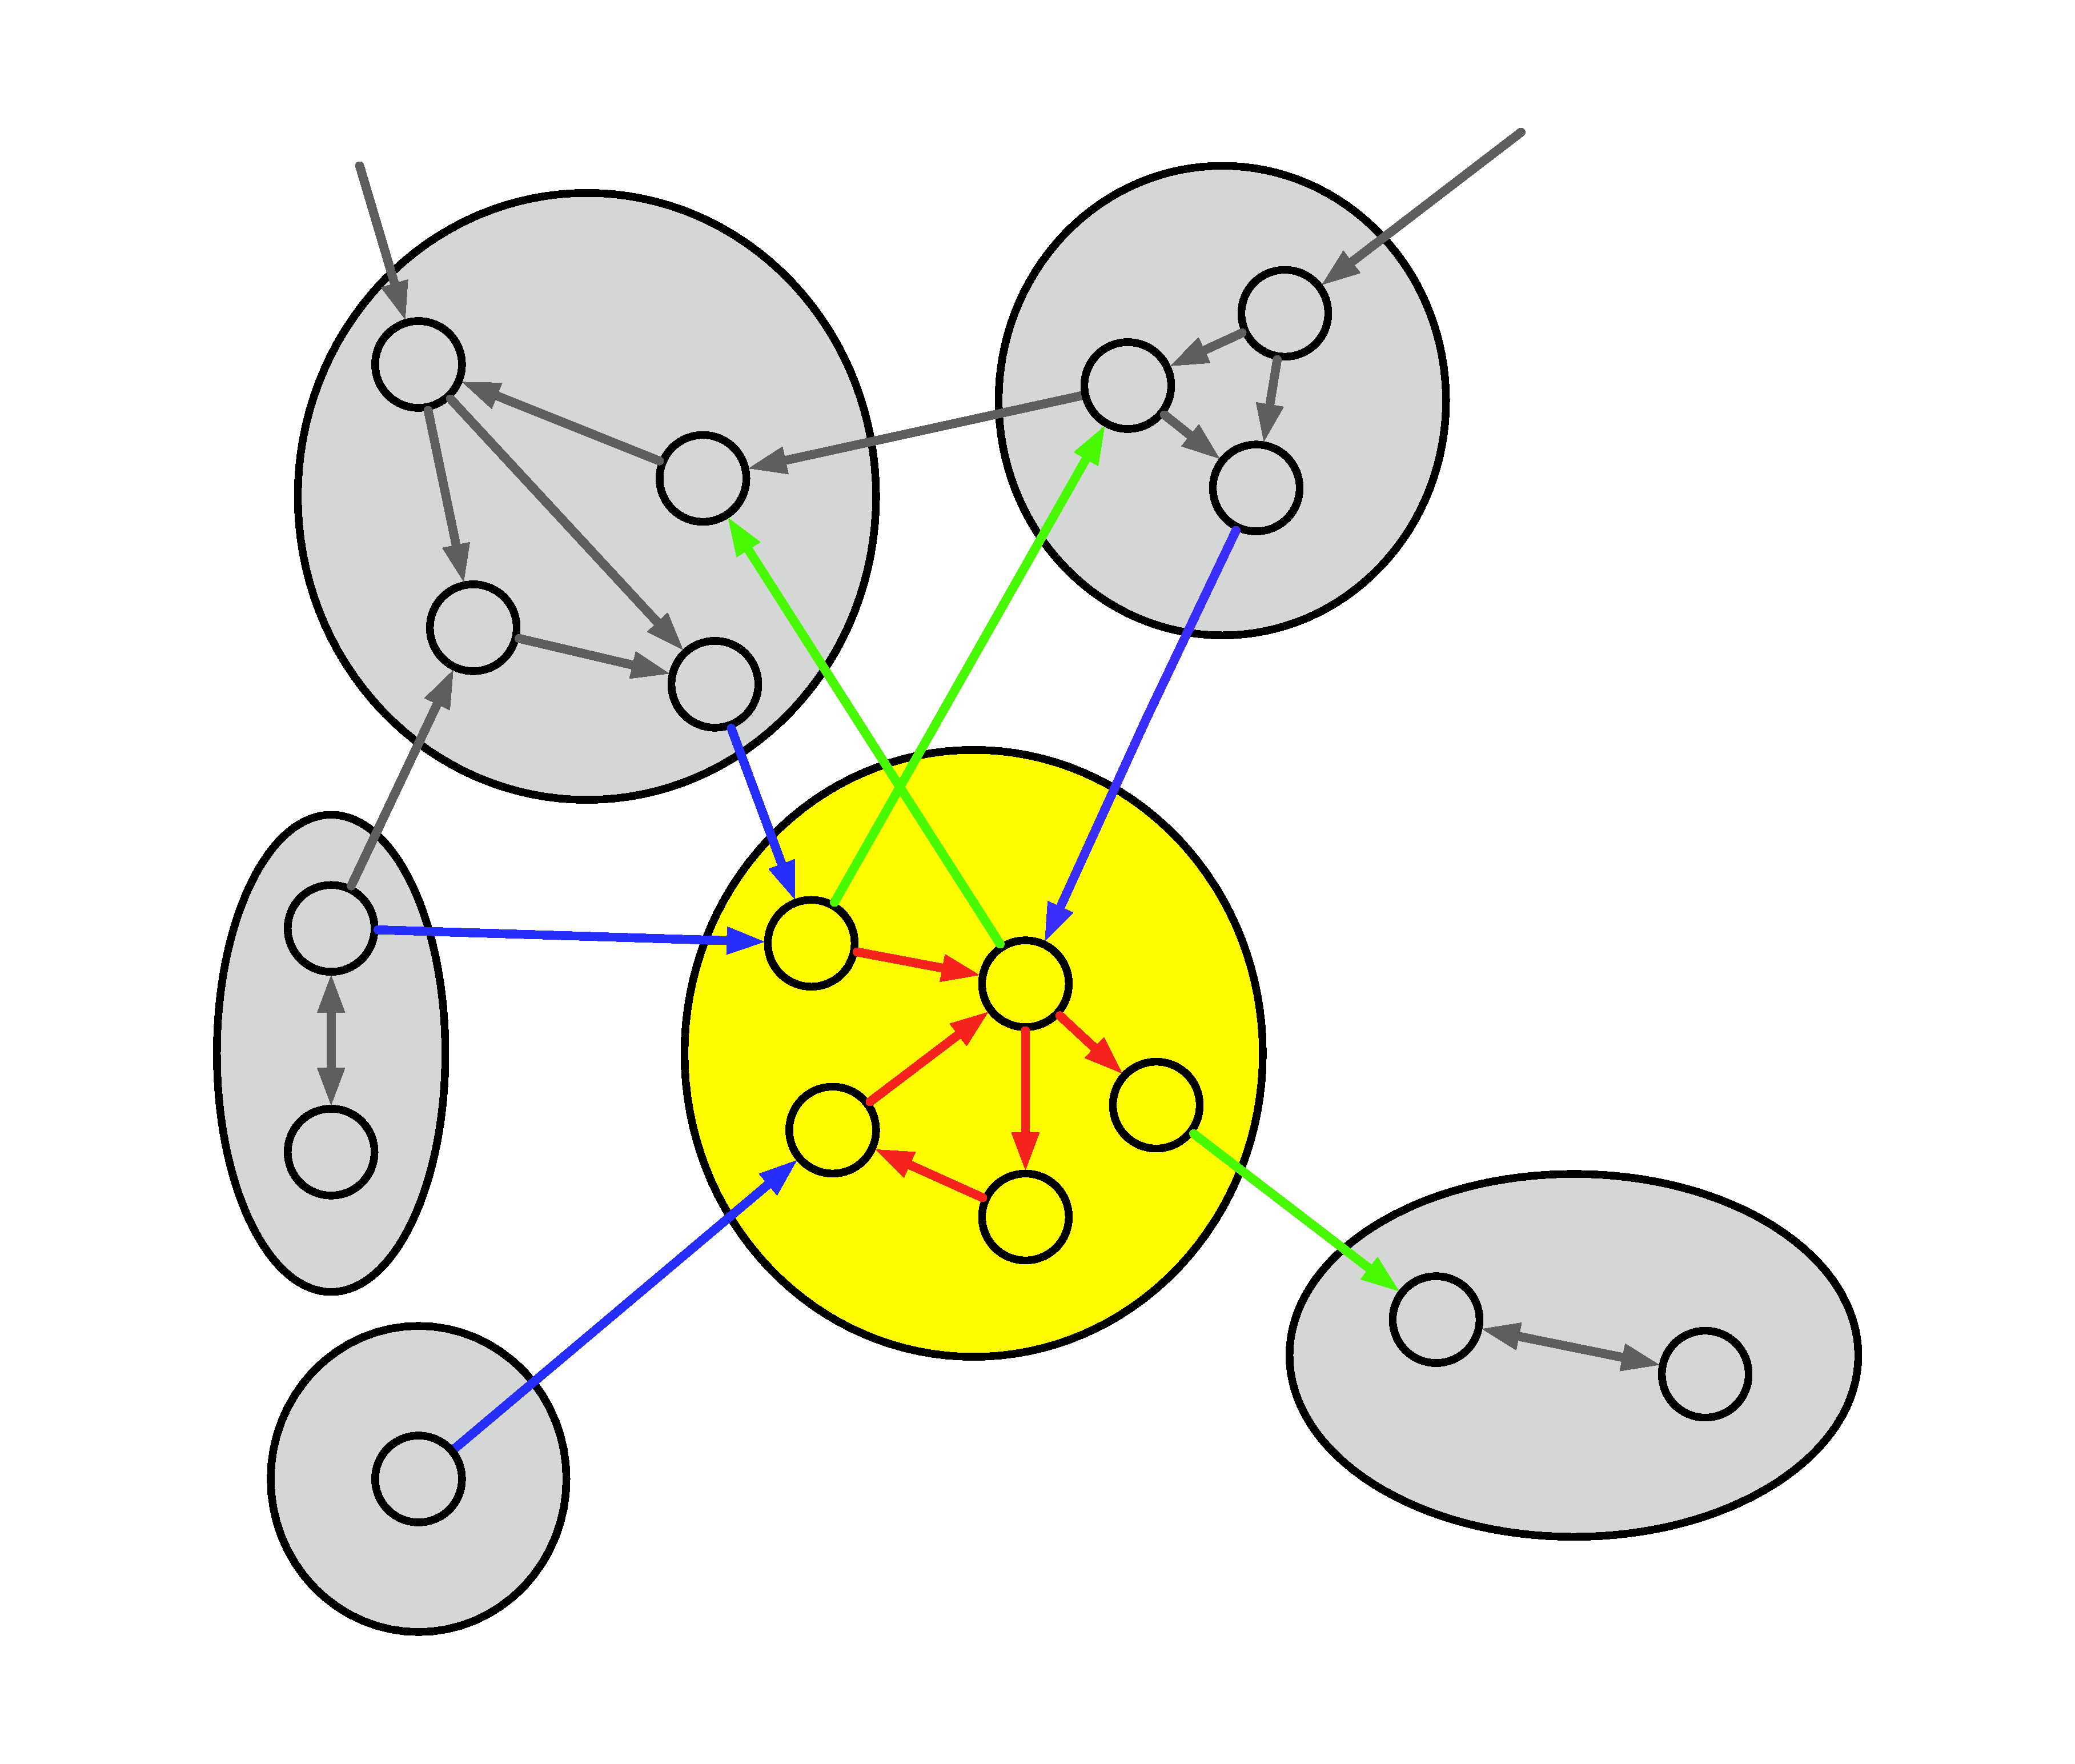
\includegraphics[width=0.50\textwidth]{figures/edge-types.eps}
\caption{An example of the edges considered in determining the edge weight distribution for a given community (the focal community is in yellow). We focus on the internal-to-internal (red), internal-to-external (green), and external-to-internal (blue) edges. For a given focal community, all other edges (grey) are not considered.}
\label{Fig-edge_types}
\end{figure}

For example, Figure~\ref{Fig-edge_types} shows the distributions of hashtag-based weights for the largest community defined by mention-retweets. We see that the distribution of internal-to-internal hashtag weights has a longer tail, with edges 

\begin{figure}[h!]
  \centering
\includegraphics[width=0.50\textwidth]{Figures/comm0_labels-mention-retweet_weights-hashtag-ecdf.pdf}
\caption{The proportion of edges with a weight at least as large as the weight on the horizontal axis, across the types of edges described in Figure~\ref{Fig-edge_types}.}
\label{Fig-dist_across_community}
\end{figure}

\begin{table}
	\caption{The median value for the ratio of the median external/internal-to-internal/external weight to median internal-to-internal weight for the different community/weight pairings.}
	\centering
	\begin{tabular}{c | c | c  c  c  c}
		& & \multicolumn{4}{ c }{Community} \\ \hline
		\multirow{4}{*}{Weight} & & S & TE & MR & HT \\ \hline
		& TE & $0.0 / 0.0$ & $0.0 / 0.0$ & $0.0 / 0.0$ & $0.0 / 0.0$\\
		& MR & $0.0 / 0.0$ & $0.0 / 0.0$ & $0.0 / 0.0$ & $0.0 / 0.0$\\
		& HT & $0.0 / 0.0$ & $0.0 / 0.0$ & $0.0 / 0.0$ & $0.0 / 0.0$
	\end{tabular}
\end{table}
\section{Conclusion and Future Work}

% What have we done:
% ==================

%In this study, we have demonstrated that the communities observed in online social %networks are highly question-dependent 
%[[Joshua:maybe reword this sentence to explicitly say what we mean by question-dependent", might be a little confusing]]
%, and that different definitions of communities reveal different relationships between users. More importantly, we have shown that these different views of the network are not revealed by using the structural network alone. We found that community structure differs across community types on both the macro (e.g. number of communities and their size distribution) and micro (e.g. specific memberships, comemberships) scale.

In this study, we have demonstrated that the communities observed in online social networks are highly question-dependent. The questions posed about a network \emph{a priori} have a strong impact on the communities observed.  Moreover, using different definitions of \emph{community} reveal different and interesting relationships between users. More importantly, we have shown that these different views of the network are not revealed by using the structural network or any one weighting scheme alone. By varying the questions we asked about the network and then deriving weighting schema to answer each question, we found that community structure differed across community types on both the macro (e.g. number of communities and their size distribution) and micro (e.g. specific memberships, comemberships) scale in interesting ways.

%We have also demonstrated that boundaries between communities represent meaningful internal/external divisions, with conversations and topics tending to be most highly concentrated within communities than without. We found this to be the case even when the communities were defined by a different criteria from the edge weights. [[Wasn't this the opposite in the transfer entropy case? Maybe I am remembering wrong. If so maybe we can spend a few sentences explaining why this is so leading into the next paragraph]]

To verify the validity of these communities we demonstrated that boundaries between communities represent meaningful internal/external divisions. In particular, conversations (e.g. retweets and mentions) and topics (e.g. hashtags) tended to be most highly concentrated within communities. We found this to be the case even when the communities were defined by a different criterion from the edge weights under study. 

% At first glance the boundaries defined by the communities in the activity-based network (those weighted with transfer entropy) seemed less meaningful. However, upon further investigation our novel use of transfer entropy for the detection of activity-based communities\footnote{It should be noted that while in previous work on online social media~\cite{ver2012information}, transfer entropy was found useful for identifying influence between users, it has not to the best of our knowledge been used to aid in the identification of communities.} brought to light a very interesting fact about this social network: influence tends to be higher across community boundaries than within them. This result echos the `strength of weak ties' theory from~\cite{granovetter1973strength}, which was supported empirically in~\cite{grabowicz2012social}. This means that our novel use of transfer entropy not only defines boundaries that are meaningful divisions between communities but it helps illustrate that influential users of a community need not be a member of that community.  

% Removed the footnote.

At first glance the boundaries defined by the activity-based communities derived from the transfer entropy weighting seemed less meaningful. However, upon further investigation our novel use of transfer entropy for the detection of activity-based communities highlighted an important fact about this social network: influence tended to be higher across community boundaries than within them. This result echos the `strength of weak ties' theory from~\cite{granovetter1973strength}, which has found empirical support in online social networks~\cite{grabowicz2012social}. This means that our use of transfer entropy not only defines boundaries that are meaningful divisions between communities but also illustrates that users who have a strong influence on a community need not be a member of that community. 


%Start of future work**
Our findings have important implications to a common problem in social network analysis: identification of influential individuals. Many network measures of influence are based on the various types of centrality (degree, betweenness, closeness, eigenvector, etc.)~\cite{newman2009networks}. Most centralities depend explicitly on the structure of the network under consideration. But we have seen in our study that a structural network alone is not sufficient to capture user interaction or influence in online social media. Thus, a na\"ive application of centrality measures to a structural network for influence detection may give rise to erroneous results. This result has been explored previously~\cite{kitsak2010identification}, and our work further highlights its importance. We believe that weighted generalizations of these centralities using transfer entropy might lead to better insights about who is actually influential in an online social network. In addition to exploring this phenomenon further, we plan to explore a broader selection of choices for both the transfer-entropy lag and tweet history time resolution. We believe that by doing an in-depth analysis of both of these parameters we can discover interesting activity-based communities that occur on much broader time scales.
%End of futre work**
  %based on methods for model selection~\cite{claeskens2008model}.

%Our work has introduced a novel use of transfer entropy for the detection of activity-based communities. 


%Our transfer entropy results thus reflect that influence tends to be higher across community boundaries than within them. This result echos the `strength of weak ties' theory from~\cite{granovetter1973strength}, which has found empirical support in~\cite{grabowicz2012social}. In addition to exploring this phenomenon further, we plan to consider more rigorous choices of both the lag and time resolution based on methods for model selection~\cite{claeskens2008model}.




% * Defined four types of communities based natural questions one might ask about users in online social media.

% * Proposed three weightings to detect such communities.

% * Demonstrated that the community structure differed between weighting to weighting.

% Future Work:
% ============

% More with transfer entropy.
% 	Why did information tend to flow *across*, rather than within, community boundaries?

% Longitudinal study:
% 	How do the different types of communities change over time? Are activity-based communities more stable than interaction-based, etc.? For example, preliminary studies indicate that `conversations,' as defined by mentions and retweets, tend to move outside of structural communities over time.

%[[This paragraph needs to be recrafted a bit. It just reads a little confusing]]

%Our work has introduced a novel use of transfer entropy for the detection of activity-based communities. In previous work on online social media~\cite{ver2012information}, transfer entropy was found useful for identifying influence between users. Our transfer entropy results thus reflect that influence tends to be higher across community boundaries than within them. This result echos the `strength of weak ties' theory from~\cite{granovetter1973strength}, which has found empirical support in~\cite{grabowicz2012social}. In addition to exploring this phenomenon further, we plan to consider more rigorous choices of both the lag and time resolution based on methods for model selection~\cite{claeskens2008model}.

% Why Care? (i.e. impact):
% ========================

% What does this mean for researchers in online social media? Businesses?

% Using concepts like centrality to determine influence 
% 	* These metrics are based solely on the structural network.
% 	* Your *activity* may be more important than your *topology* in determining
% 	  your influence.
%[[While I agree with this next paragraph completely I am not sure we covered this topic enough to be the final paragraph of the conclussion or even in the conclusion. I need to think about this...]]

% More generally, our work demonstrates that asking the proper question is an unavoidable first step to community detection, and that the rich data sets available from 

This work demonstrates that asking the proper question and then crafting an appropriate weighting scheme to answer that question is an unavoidable first step for community detection in online social media. More generally, this work illustrates that without a clear definition of community, many rich and interesting communities present in online social networks remain invisible. Question-oriented community detection can bring those hidden communities into the light.



\section{Funding}
%Elisa Omodei is partially supported by a PhD grant from the R\'{e}gion \^{I}le-de-France (DIM 2011) and by the French National Agency of Research (ANR) through the grant Algopol (ANR-12-CORD-0018).
This work was partially supported by the R\'{e}gion \^{I}le-de-France [DIM 2011 to E.O.]; and by the French National Agency of Research [ANR-12-CORD-0018 to E.O.].
%We are grateful to DARPA for the support of David Darmon.

\section{Acknowledgments}

Thanks to Cesar Flores, Lu\'is Seoane, Kevin Stadler, Jody Wright, and Nix Barnett for their contributions to preliminary ideas related to this paper and to Michelle Girvan, William Rand, Aaron Clauset, and Ryan James for their valuable comments and suggestions, and the
anonymous reviewers whose comments strengthened the
presentation. Finally, we would like to acknowledge the Santa Fe Institute and its Complex Systems Summer School for providing the intellectually stimulating environment where this project began.


\appendix

\section{Appendix A: Transfer Entropy and Its Estimation from Data}

Let $\{X_{t}\}$ and $\{ Y_{t}\}$ be two strong-sense stationary stochastic processes\footnote{Recall that a stochastic process is strong-sense stationary if the joint distribution for the process evaluated at finitely many time points is invariant to an overall timeshift~\cite{grimmett2001probability}.}. In our work, these would correspond to the activities, $X_{t}(u)$ and $X_{t}(v),$ of two users $u$ and $v$. We use the notation $X_{t-k}^{t}$ to denote the values of the stochastic process from time $t-k$ to time $t$, $X_{t-k}^{t} = (X_{t-k}, X_{t-(k-1)}, \ldots, X_{t - 1}, X_{t})$. The lag-$k$ transfer entropy~\cite{schreiber2000measuring} of $Y$ on $X$ is defined as 
\begin{align}
	\text{TE}_{Y \to X}^{(k)} &= H\left[X_{t} | X_{t-k}^{t-1}\right] - H\left[X_{t} | X_{t-k}^{t-1}, Y_{t-k}^{t-1}\right], \label{Eqn-TE}
\end{align}
where
\begin{align}
	H\left[X_{t} | X_{t-k}^{t-1}\right] = - E\left[ \log_{2} p(X_{t} | X_{t-k}^{t-1}) \right]
\end{align}
and 
\begin{align}
	H\left[X_{t} | X_{t-k}^{t-1}, Y_{t-k}^{t-1}\right] = - E\left[ \log_{2} p(X_{t} | X_{t-k}^{t-1}, Y_{t-k}^{t-1}) \right]
\end{align}
are the usual conditional entropies over the conditional (predictive) distributions $p(x_{t} | x_{t-k}^{t-1})$ and $p(x_{t} | x_{t-k}^{t-1}, y_{t-k}^{t-1})$. This formulation was originally developed in~\cite{schreiber2000measuring}, where transfer entropy was proposed as an information theoretic measure of \emph{directed} information flow. Formally, recalling that $H\left[X_{t} | X_{t-k}^{t-1}\right]$ is the uncertainty in $X_{t}$ given its values at the previous $k$ time points, and that $H\left[X_{t} | X_{t-k}^{t-1}, Y_{t-k}^{t-1}\right]$ is the uncertainty in $X_{t}$ given the joint process $\{(X_{t}, Y_{t})\}$ at the previous $k$ time points, transfer entropy measures the reduction in uncertainty of $X_{t}$ by including information about $Y_{t-k}^{t-1},$ controlling for the information in $X_{t - k}^{t-1}$. By the `conditioning reduces entropy' result~\cite{cover2012elements}
\begin{align}
	H[X | Y, Z] \leq H[X | Y],
\end{align}
we can see that transfer entropy is always non-negative, and is zero precisely when $H\left[X_{t} | X_{t-k}^{t-1}\right] = H\left[X_{t} | X_{t-k}^{t-1}, Y_{t-k}^{t-1}\right]$, in which case knowing the past $k$ lags of $Y_{t}$ does not reduce the uncertainty in $X_{t}$. If the transfer entropy is positive, then $\{ Y_{t}\}$ is considered causal for $\{ X_{t}\}$ in the Granger sense~\cite{granger1963economic}.

In estimating the transfer entropy from finite data, we will assume that the process $\{(X_{t}, Y_{t})\}$ is jointly stationary, which gives us that
\begin{align}
	p(x_{t} | x_{t-k}^{t-1}) = p(x_{k+1} | x_{1}^{k})
\end{align}
and
\begin{align}
	p(x_{t} | x_{t-k}^{t-1}, y_{t-k}^{t-1}) = p(x_{k+1} | x_{1}^{k}, y_{1}^{k})
\end{align}
for all $t$. That is, the predictive distribution only depends on the past, not on when the past is observed. Given this assumption, we compute estimators for $p(x_{k+1} | x_{1}^{k})$ and $p(x_{k+1} | x_{1}^{k}, y_{1}^{k})$ by `counting': for each possible marginal and joint past $x_{1}^{k}$ and $(x_{1}^{k}, y_{1}^{k})$, we count the number of times a future of type $x_{k+1}$ occurs, and normalize to obtain the appropriate estimators of the one-step-ahead predictive distributions. Call these estimators $\hat{p}(x_{k+1} | x_{1}^{k})$ and $\hat{p}(x_{k+1} | x_{1}^{k}, y_{1}^{k})$. Then the plug-in estimator for the transfer entropy is
\begin{align}
	\widehat{\text{TE}}_{Y \to X}^{(k)} &= \hat{H}\left[X_{t} | X_{t-k}^{t-1}\right] - \hat{H}\left[X_{t} | X_{t-k}^{t-1}, Y_{t-k}^{t-1}\right]
\end{align}
where we use the plug-in estimators $\hat{H}\left[X_{t} | X_{t-k}^{t-1}\right]$ and $\hat{H}\left[X_{t} | X_{t-k}^{t-1}, Y_{t-k}^{t-1}\right]$ for the entropies. It is well known that the plug-in estimator for entropy is biased~\cite{paninski2003estimation}. To account for this bias, we use the Miller-Madow adjustment to the plug-in estimator~\cite{miller1955note}. For a random variable $X$ taking on finitely many values from an alphabet $\mathcal{X}$, the Miller-Madow estimator is
	\begin{align}
		\tilde{H}[X] = \hat{H}[X] + \frac{|\hat{\mathcal{X}}| - 1}{2 n}
	\end{align}
	where $|\mathcal{\hat{X}}|$ is the number of observed symbols from the alphabet $\mathcal{X}$ and $n$ was the number of samples used to estimate $\hat{H}[X].$ The definition of transfer entropy~(\ref{Eqn-TE}) can be rewritten in terms of joint entropies as
	\begin{align}
		TE_{Y \to X}^{(k)} &= H[X_t | X_{t-k}^{t-1}] - H[X_t | X_{t-k}^{t-1},Y_{t-k}^{t-1}] \\ 
		&= H[X_t,X_{t-k}^{t-1}]-H[X_{t-k}^{t-1}]-H[X_t,X_{t-k}^{t-1},Y_{t-k}^{t-1}]+H[X_{t-k}^{t-1},Y_{t-k}^{t-1}],
	\end{align}
	We then apply the Miller-Madow adjustment individually to each of the entropy terms. For example, for the first term, we have
	\begin{align}
		\tilde{H}[X_{t}, X_{t - k}^{t-1}] = \tilde{H}[X_{t - k}^{t}] = \hat{H}[X_{t-k}^{t}] + \frac{|\widehat{\mathcal{X}^{k+1}}| - 1}{2n},
	\end{align}
	where $|\widehat{\mathcal{X}^{k+1}}|$ is the number of $(k + 1)$-tuples we actually observe (of the $2^{k + 1}$ possible tuples). Doing this for each term, the overall Miller-Madow estimator for the transfer entropy is
	\begin{align}
		\widetilde{TE}_{Y \to X}^{(k)} &= \tilde{H}[X_t | X_{t-k}^{t-1}] - \tilde{H}[X_t | X_{t-k}^{t-1},Y_{t-k}^{t-1}] \\ 
		&= \tilde{H}[X_t,X_{t-k}^{t-1}]-\tilde{H}[X_{t-k}^{t-1}]-\tilde{H}[X_t,X_{t-k}^{t-1},Y_{t-k}^{t-1}]+\tilde{H}[X_{t-k}^{t-1},Y_{t-k}^{t-1}].
	\end{align}
	One possible problem with this estimator is that it can result in \emph{negative} estimates of entropies. That usually occurs when $\hat{H}$ is very small. In these cases, we truncate set the estimator to zero.

%\section{Appendix B: Comparing Edges Across Different Community Types}



\bibliographystyle{comnet}
%\bibliographystyle{plainnat}
\bibliography{references.bib}


% %File: formatting-instruction.tex
\documentclass[letterpaper]{article}
\usepackage{aaai}
\usepackage{times}
\usepackage{helvet}
\usepackage{courier}
\usepackage{amssymb, amsmath, amsthm}
\usepackage{graphicx}
\frenchspacing
\setlength{\pdfpagewidth}{8.5in}
\setlength{\pdfpageheight}{11in}
\pdfinfo{
/Title (Input Your Paper Title Here)
/Author (John Doe, Jane Doe)
/Keywords (Input your paper keywords in this optional area)}

%%%%%%%%%%
% Section Numbers
% Uncomment if you want to use section numbers % and change the 0 to a 1 or 2
\setcounter{secnumdepth}{0}

%%%%%%%%%%
% Body of Paper Begins
\begin{document}

% Title, Author, and Address Information
\title{
%Followers are not enough: Beyond structure in the detection of communities \\
Followers are not enough: Exploring the communities that exist beyond structure \\
%Followers are not enough: Activity, Interaction, and Topic-based Communities in Online Social Networks \\
%Followers are not enough: Beyond structural communities in online social networks
% \\
 %Followers are not enough: exploring communities beyond structure
 }
%   \author{David Darmon  \\
%  University of Maryland\\
% Dept. of Mathematics \\
% ddarmon@math.umd.edu \\
%  \And Elisa Omodei \\
%  LaTTiCe (CNRS, ENS, Paris 3)\\
% ISC-PIF\\
% elisa.omodei@ens.fr \\
%  \And 
%  Joshua Garland\\
%  University of Colorado at Boulder\\
% Dept. of Computer Science \\
% joshua.garland@colorado.edu}

\maketitle

\begin{abstract}
\begin{quote}
[[Joshua]]

[[David]]

[[Elisa]]

\end{quote}
\end{abstract}

\section{Introduction}

Networks play a central role in online social media services like Twitter, Facebook, and Google+. These services allow a user to interact with others based on the online social network they curate through a process known as contact filtering~\cite{cazabet2012automated}. For example, `friends' on Facebook represent reciprocal links for sharing information, while `followers' on Twitter allow a single user to broadcast information in a one-to-many fashion. Central to all these interactions is the fact that the \emph{structure} of the social network influences how information can be broadcast or diffuse through the service.

Because of the importance of structural networks in online social media, a large amount of work in this area has focused on using structural networks for community detection. In this traditional view, `community' is defined as a collection of nodes (users) within the network which are more highly connected to each other than to nodes (users) outside of the community 
%Here, by `community' we mean the standard definition from the literature on social networks: a collection of nodes (users) within the network which are more highly connected to each other than to nodes (users) outside of the community
~\cite{girvan2002a, newman2004finding}. For instance, in~\cite{java2009we}, the authors use a follower network to determine communities within Twitter, and note that conversations tend to occur within these communities. The approach of focusing on the structure of networks makes sense for `real-world' sociological experiments, where obtaining additional information about user interactions may be expensive and time-consuming. However, with the prevalence of large, rich data sets for online social networks, additional information beyond the structure alone may be incorporated, and these augmented networks more realistically reflect how users interact with each other on social media services~\cite{nguyen2011adaptive},~\cite{grabowicz2012social}.

%A large body of work exists on methods for automatic detection of communities within networks~\cite{newman2004fast,newman2004finding,rosvall2008maps,blondel2008fast,LancichinettiPlos}. See~\cite{fortunato2010community} for a recent review. 
A large body of work exists on methods for automatic detection of communities within networks, {\it e.g.,} the stochastic blockmodel~\cite{Holland1983} (and its recent generalization to weighted networks~\cite{Aicher26062014}), the \DIFdelbegin \DIFdel{Newman and Girvan }\DIFdelend \DIFaddbegin \DIFadd{Girvan-Newman }\DIFaddend algorithm~\cite{newman2004finding}, clique percolation~\cite{PalEtAl05}, Infomap~\cite{Rosvall08mapsof}, Louvain~\cite{blondel2008fast}, and the recently introduced OSLOM~\cite{LancichinettiPlos}.
All these methods \DIFdelbegin \emph{\DIFdel{begin}} %DIFAUXCMD
\DIFdelend \DIFaddbegin \DIFadd{begin }\DIFaddend with a given network, and then attempt to uncover structure present in the network, \DIFdelbegin \DIFdel{i.e., }\DIFdelend \DIFaddbegin \emph{\DIFadd{i.e.,}} \DIFaddend they are agnostic to how the network was constructed. As opposed to this agnostic analysis, we \DIFdelbegin \DIFdel{propose and }\DIFdelend \DIFaddbegin \DIFadd{propose---and }\DIFaddend illustrate the importance \DIFdelbegin \DIFdel{of a question-focused }\DIFdelend \DIFaddbegin \DIFadd{of---a }\emph{\DIFadd{multifaceted question-focused}} \DIFaddend approach. We believe that in order to understand \DIFaddbegin \DIFadd{all of }\DIFaddend the communities present in a \DIFdelbegin \DIFdel{data set}\DIFdelend \DIFaddbegin \DIFadd{network}\DIFaddend , it is important to \DIFdelbegin \DIFdel{begin with a clear picture }\DIFdelend \DIFaddbegin \DIFadd{take the following crucial steps: 
}\begin{enumerate}

\item \DIFadd{Ask }\emph{\DIFadd{several}} \DIFadd{questions about the communities that may be present in the network, each of which is aimed at revealing a new facet }\DIFaddend of the community \DIFdelbegin \DIFdel{type under consideration---}\DIFdelend \DIFaddbegin \DIFadd{present in the network---}\DIFaddend {\it e.g.,} \DIFdelbegin \DIFdel{are we looking for groups of friends? or for groups of people having a common interest?
---and }\DIFdelend \DIFaddbegin \DIFadd{which users are tightly connected structurally? which groups of users have similar topical interests?
}

\item \DIFadd{Derive a weighting scheme aimed at answering each of the questions asked in the first step and }\DIFaddend then perform community detection \DIFdelbegin \DIFdel{with that community type in mind. 
}\DIFdelend \DIFaddbegin \DIFadd{on each weighted network.
}\item \DIFadd{Compare the disjoint }\emph{\DIFadd{and}} \DIFadd{overlapping communities that arise from this series of experiments on a micro and macro scale to unveil all the interesting facets of community present in the social network. 
}\end{enumerate}
\DIFaddend 

This is especially true for social network analysis. In \DIFdelbegin \DIFdel{online }\DIFdelend social networks, a `community' could refer to several possible structures. The simplest definition of community, as we have seen, might stem from the network of explicit connections between users on a service (friends, followers, etc.). On small time scales, these connections are more or less static, and we might instead determine communities\DIFaddbegin \DIFadd{, as is standard in the literature}\alert{david or elisa can you add some citations please}\DIFadd{\mbox{%DIFAUXCMD
\cite{}
}%DIFAUXCMD
, }\DIFaddend based on who is talking to whom \DIFaddbegin \DIFadd{or which users talk about similar topics}\DIFaddend , providing a more dynamic picture \DIFdelbegin \DIFdel{. On a more abstract level, a user might consider themselves part of a communityof people discussing similar topics.
We might also }\DIFdelend \DIFaddbegin \DIFadd{of community.
More abstractly, we could even }\DIFaddend define communities as \DIFdelbegin \DIFdel{collections }\DIFdelend \DIFaddbegin \DIFadd{groups }\DIFaddend of people who exhibit similar activity profiles\DIFdelbegin \DIFdel{and seem to ``influence" each other's activity on the network}\DIFdelend . We can characterize these types of communities based on the types of questions we might ask about them:
\begin{itemize}
	\item \textbf{Structure-based:} Who are your stated friends? Whom do you follow?
	\item \textbf{Activity-based:} \DIFdelbegin \DIFdel{Whose activity influences your activity}\DIFdelend \DIFaddbegin \DIFadd{Who shares similar activity profiles}\DIFaddend ?
	\item \textbf{Topic-based:} What do you talk about?
	\item \textbf{Interaction-based:} Whom do you communicate with?
\end{itemize}

This is not meant to be an exhaustive list, but rather a list of some of the more common types of communities observed \DIFaddbegin \DIFadd{and studied }\DIFaddend in social networks. \DIFdelbegin \DIFdel{We }\DIFdelend \DIFaddbegin \DIFadd{Instead of looking at each of these questions in isolation---which is the standard approach---we }\DIFaddend propose looking at when\DIFaddbegin \DIFadd{, why, }\DIFaddend and how communities motivated by these different questions overlap \DIFaddbegin \DIFadd{and are disjoint}\DIFaddend , and whether different approaches to asking the question, ``What community are you in?'' leads to different insights about a social network. For example, a user on Twitter might connect mostly with computational social scientists, utilize the service nearly every time a particular user or group of users is active, talk mostly about machine learning, and interact solely with close friends (who may or may not be computational social scientists). 
\DIFdelbegin \DIFdel{Each of these different `profiles' of the userhighlight different views of the user's social network, and represent different types of communities. We divide our approaches into four categories based on }\DIFdelend \DIFaddbegin \DIFadd{For this user, the answers to each question therefore correspond to more or less distinct communities. By contrast, a teenage user may only connect and interact with their friends, will most likely exhibit similar activity patterns dictated by the academic and extracurricular schedule of a student. For this user, the answers to each question map to the same community of users.
Thus, each question acts to highlight a particular `profile' of a user, and these profiles can help identify the ways in which a user interacts with and like other users in their online social network. 
We now consider in more detail how each of these types of questions motivates a question-specific community. Later in Section~\ref{sec:conc} we will show how asking }\emph{\DIFadd{all}} \DIFadd{of these questions---instead of focusing on only one---gives a much deeper multifaceted view of the overlapping }\emph{\DIFadd{and}} \DIFadd{disjoint communities that users belong to. 
}

\DIFadd{Na\"ively }\DIFaddend the \DIFdelbegin \DIFdel{questions outlined above: structure-based, }\DIFdelend activity-based \DIFdelbegin \DIFdel{, topic-based, and interaction-based. 
The structure-based approach, as outlined above, is most common, and for our data relies on reported follower relationships.
}%DIFDELCMD < 

%DIFDELCMD < %%%
\DIFdel{The activity-based }\DIFdelend approach is motivated by the question of ``Which \DIFdelbegin \DIFdel{user's activity `influences' the activity of another user}\DIFdelend \DIFaddbegin \DIFadd{users in a network have similar activity profiles}\DIFaddend ?"
%DIF < , \emph{i.e.}, which user(s) cause a user(s) to interact with the network. 
 %DIF > --- \emph{i.e.,} which user(s) cause groups of users to become active on the network.  %, \emph{i.e.}, which user(s) cause a user(s) to interact with the network. 
 With this question in mind, a community can then be thought of as those \DIFdelbegin \DIFdel{individuals who ``influence}\DIFdelend \DIFaddbegin \DIFadd{users who use (or do not use) the service at similar times. However, the measure we use is slightly more subtle that this. In particular, these communities can be thought of as groups of users who possess so-called ``predictive capacity}\DIFaddend " \DIFdelbegin \DIFdel{each other's activity on the network. In general, quantifying the influence of one user on anotheris a difficult and ill-understood problem. For that reason, we focus on a smaller subset of that problem, }\emph{\DIFdel{viz.}}%DIFAUXCMD
\DIFdel{, quantifying influence purely from an information theoretic framework. 
%DIF < The primary tool for answering this question is the  For this approach
%DIF < \alert{Maybe add a sentence hedging influence}
}\DIFdelend \DIFaddbegin \DIFadd{with one another, i.e., given a user $u$ and follower $f$ who are members of a community detected with this weighting, there exists a reduction in uncertainty about the activity profile of follower $f$ (tweeting or remaining silent), given the tweet history of user $u$. 
}\DIFaddend 

To accomplish this, we consider each user on Twitter as an information processing unit, but completely ignore the \emph{content} of their tweets. We then weight the directed edges (the reported follower-followee relationships) between users with the so-called \emph{transfer entropy} introduced in~\cite{schreiber2000measuring}.  Transfer entropy is an information theoretic measure of \emph{directed} information flow. \DIFdelbegin \DIFdel{It has been shown in~\mbox{%DIFAUXCMD
\cite{ver2012information}
}%DIFAUXCMD
that a positive transfer entropy between a user $u$ and a follower $f$ indicates that $u$ ``influences" $f$, or that $u$ and $f$ share a common influencer. In particular, }\DIFdelend \DIFaddbegin \DIFadd{Since transfer entropy is a nonlinear generalization of Granger causality \mbox{%DIFAUXCMD
\cite{granger1963economic}
}%DIFAUXCMD
, we assume---as is standard---a }\DIFaddend positive transfer entropy from the tweet history of a user $u$ to a follower $f$'s tweet history implies that this relationship is causal in the Granger sense\DIFdelbegin \DIFdel{~\mbox{%DIFAUXCMD
\cite{granger1963economic}
}%DIFAUXCMD
.  }\DIFdelend \DIFaddbegin \DIFadd{.  Thus, communities detected in this way have members whose tweet histories are causally related in a Granger sense. }\DIFaddend As a result, transfer entropy is often thought of as a measure of ``influence" in an information theoretic sense. 
\DIFdelbegin \DIFdel{Thus, communities detected in this way have members whose tweet histories are causally related in a Granger sense, }\emph{\DIFdel{i.e.}}%DIFAUXCMD
\DIFdel{, members who ``influence}\DIFdelend \DIFaddbegin 

\DIFadd{According to~\mbox{%DIFAUXCMD
\cite{ver2012information}
}%DIFAUXCMD
a positive transfer entropy between a user $u$ and a follower $f$ indicates that $u$ ``influences}\DIFaddend " \DIFdelbegin \DIFdel{each others activity on the network. %DIF < Obviously the concept of ``influence" is extremely broad and quantifying influence in a social network is neither well understood nor well defined in the literature. 
}%DIFDELCMD < 

%DIFDELCMD < %%%
\DIFdel{We want to reiterate that we do not imply that this information theoretic measure completely }\DIFdelend \DIFaddbegin \DIFadd{$f$, or that $u$ and $f$ share a common influencer. We would like to point out however that we are skeptical whether this measure truly }\DIFaddend captures social influence in \DIFdelbegin \DIFdel{general. However, we conjecture, it does capture a useful subset of that relationship. In this paper, when we say }\emph{\DIFdel{influence}} %DIFAUXCMD
\DIFdel{we explicitly refer to }\DIFdelend \DIFaddbegin \DIFadd{its entirety. We instead treat this weighting as a way to explicitly quantify }\DIFaddend a reduction in uncertainty of whether a follower $f$ will be active or not given the \DIFdelbegin \DIFdel{past }\DIFdelend \DIFaddbegin \DIFadd{tweet }\DIFaddend history of a user $u$. \DIFdelbegin \DIFdel{We will however show }\DIFdelend \DIFaddbegin \DIFadd{This provides an information theoretic framework in which we can capture communities with predictive capacity between users or users with similar activity profiles. We call this relation ``PV-AC". As an aside, while we are skeptical that this measure can capture social influence, }\DIFaddend later in this paper \DIFaddbegin \DIFadd{we show }\DIFaddend that this information theoretic measure \DIFdelbegin \DIFdel{of influence }\DIFdelend agrees with other concepts of influence such as the Forbes list of ``Top 10 Social Media Influencers" and corroborates with the so-called strength of weak ties~\cite{granovetter1973strength}. \DIFaddbegin \DIFadd{Even so, we do not explicitly treat---and we do not believe it should be treated---as a quantification of social influence. Instead this measure should be treated merely as a way to suggest users with casually related (in a Granger sense) tweet histories, i.e., users with similar activity profiles (PV-AC).
}\DIFaddend 


%DIF < emphasize that we are not saying these casual relationships necessarily suggest social or \alert{?? } influence, but simply a casual re. In this paper when we say that a user $u$ influences a user $f$ we simply mean that there is a reduction in uncertanity about whether user $u$ will be active or not given the past history of user $f$. We will show that this information theoretic view of influence is a useful and
%DIF < Effectively, if there is a positive transfer entropy from user $u$ to $v$ then there is a reduction in uncertainty about user \alert{$u$/$v$} tweeting given the recent tweet history of user \alert{$u$/$v$}. This can and has been interpreted as a form of influence, if user \alert{$u$/$v$} reduces the uncertainty about \alert{$u$/$v$} tweeting then it may be the case that this was a form of social influence. We are fully aware that the difference between information theoretic and social influence are different but think this may be an interesting area to explore. Later we show that using this measure alone we can detect ``influential users" who are also listed as \alert{Forbes ...}. We instead treat this weighting as a way to quantify which users activity are quantified by each other, i.e., communities that use twitter in similar ways.
%DIF < A positive value for the transfer entropy of the user $u$ on $f$ indicates that $u$ influences $f$, or that $u$ and $f$ share a common influencer~\cite{ver2012information}. $T_{u \to f}$
%DIF < think this paragrpah should be something like we use it as a way to quantify activity but we think it may have applicaitons in influence detection for example if one user has high transfer entropy with an entire community, then this may imply that user has strong social influence on the activity of a given community defined with this weighting scheme. For example, Denver Broncos tweet that they fired John Elway and an entire network of Broncos fans begins tweeting this may be a rank of influence. 
\DIFdelbegin %DIFDELCMD < 

%DIFDELCMD < %%%
\DIFdelend This activity-based approach was motivated by a method used by Shalizi \emph{et al.} in ~\cite{shalizi2007discovering} to detect functional communities within populations of neurons, but to the best of our knowledge, this is the first use of transfer entropy for community detection in online social networks. Various other information theoretic approaches have been used successfully to analyze online social networks, \emph{e.g.,} to gain insight into local user behavior~\cite{darmon2013understanding}, to detect communities based on \emph{undirected} information flow~\cite{darmon2013detecting}, and to perform network inference and link prediction~\cite{ver2012information}.
%DIF < While various information theoretic measures has been applied previously to the analysis of networks arising in online social media~\cite{ver2012information,darmon2013detecting}, 


\DIFdelbegin \DIFdel{Our }\DIFdelend \DIFaddbegin \DIFadd{The }\DIFaddend topic-based and interaction-based approaches, in contrast to the activity-based approach, rely on the \emph{content} of a user's interactions and ignore their temporal components. The content contains a great deal of information about communication between users.
There are two broad approaches to topic-based communities in the literature. \cite{rossi2012conversation} used a set of users collected based on their use of a single hashtag, and tracked the formation of follower and friendship links within that set of users. In~\cite{lim2012following}, the authors chose a set of topics to explore, and then seeded a network from a celebrity chosen to exemplify a particular topic. Both approaches thus begin with a particular topic in mind, and perform the data collection accordingly. Other approaches use probabilistic models for the topics and treat community membership as a latent variable~\cite{yin2012latent}.
For example, a popular approach to analyzing social media data is to use Latent Dirichlet Allocation (LDA) to infer topics based on the prevalence of words within a status~\cite{zhao2011comparing,michelson2010discovering}. The LDA model can then be used to infer distributions over latent topics, and the similarity of two users with respect to topics may be defined in terms of the distance between their associated topic distributions. Because our focus is not on topic identification, we apply a simpler approach using hashtags as a proxy for topics \DIFaddbegin \DIFadd{similar to the approaches presented in}\DIFaddend ~\cite{becker2011beyond,tsur2012s}. We can then define the similarity of two users in terms of their hashtags, and use this similarity to build a topic-based network.

Finally, the interaction-based approach relies on the meta-data and text of messages to identify whom a user converses with on the social media service. On Twitter, we can use mentions (indicating a directed communication) and retweets (indicating endorsement of another user) to identify conversation. 
\DIFdelbegin \DIFdel{Moreover, we can define a directed influence between two users by considering the attention paid to that user compared to all other users. This allows us to generate a network based on conversations and user interactions.
}\DIFdelend A few works have investigated this type of community. For example, \cite{conover2011political} considered both mention and retweet networks in isolation for a collection of users chosen for their political orientation. In~\cite{deitrick2013mutually}, the authors construct a dynamic network based on simple time-windowed counts of mentions and retweets, and use the evolution of this network to aid in community detection.

Previous research on communities in social networks focused almost exclusively on different network types in isolation.
A notable exception to the analysis of isolated types of communities is~\cite{lim2012tweets}, that considered both structure-based and interaction-based communities on Twitter. However, this study focused on data collected based on particular topics (country music, tennis, and basketball), and not on a generic subpopulation of Twitter users. Moreover, it did not explore the differences in community structure resulting from the different network weightings, and focused on aggregate statistics (community size, network statistics, etc.). Another notable exception is~\cite{kao2013talison}, where the authors used a tensor representation of user data to incorporate retweet and hashtag information into a study of the social media coverage of the Occupy Movement. The tensor can then be decomposed into factors in a generalization of the singular value decomposition of a matrix, and these factors can be used to determine `salient' users. However, this approach focused on data for a particular topic (the Occupy Movement) and did not collect users based on a structural network.

\DIFdelbegin \DIFdel{The }\DIFdelend \DIFaddbegin \DIFadd{Studying how the communities derived from follower-followee, }\DIFaddend activity-based, topic-based, and interaction-based networks \DIFdelbegin \DIFdel{allow us to build }\DIFdelend \DIFaddbegin \DIFadd{are disjoint as well as overlapping allow for }\DIFaddend a more complete picture of the \emph{implicit} networks present in online social media, as opposed to the \emph{explicit} social network indicated by \DIFdelbegin \DIFdel{structural links }\DIFdelend \DIFaddbegin \DIFadd{follower links alone}\DIFaddend . In this paper, we explore the relation between these various possible networks and their corresponding communities. We begin by describing the methodologies used to generate the various types of networks, and infer their community structure.  We then explore how the communities of users differ depending on the type of network used. Finally, we explore how communication patterns differ across and within the different community types. \DIFdelbegin %DIFDELCMD < 

%DIFDELCMD < %%%
\DIFdelend \DIFaddbegin \DIFadd{We conclude by illustrating that this multifaceted question-oriented approach to community detection provides interesting insight into the intricate multifaceted structure of several different users' communities; information that would not be available if only a single form of community detection was performed. 
}\DIFaddend %\section{Related Work}

% Structural:
% ==========

% \cite{java2009we} Determine friendship network on Twitter to define communities.

% \cite{nguyen2011adaptive} Uses a dynamic community detection algorithm (that uses snapshots of the network), but still focuses on \emph{structural} ties (Facebook friendship relationships)

% Interaction-based:
% ==================

% \cite{deitrick2013mutually} use 'dynamic' mention-retweet network to detect communities, but just augment the count of mentions retweets in the weighting (instead of using a proportion), and don't combine mentions and retweets.

% \cite{conover2011political} Retweet-mention analysis for political polarization analysis
% http://truthy.indiana.edu/site_media/pdfs/conover_icwsm2011_polarization.pdf

% Activity-based:
% ===============

% None, to the best of our knowledge.

% Topic-based:
% ============

% \cite{lim2012following} "We propose an efficient approach for detecting communities that share common interests on Twitter, based on linkages among followers of celebrities representing an interest category." Use both InfoMAP and clique percolation.

% \cite{rossi2012conversation} Collect users who use the same hashtag (a *single* hashtag, #XF5, for XFactor 5), and then note if this impacts the friend/follower network.

% \cite{xu2011sentiment} Generate 'sentiment' networks.

% Most-relevant:
% ==============

% \cite{lim2012tweets} This one is *very* important: they also note that structural links do not indicate communication. They use an interaction-based approach (mentions only). But they do not use a weighted version of the structural network. Instead, they use . And they do not go into much depth comparing how the two types of communities (structural and activity-based) differ. Moreover, they explicitly seed their network to focus around a particular topic (country music, tennis, basketball, etc.)

\section{Content-Free v\@. Content-Full Communities}

Lorem ipsum.
\section{Methodology}

\subsection{Community Detection}

Lorem ipsum.

\subsection{Activity-Based Communities and Transfer Entropy}

Suppose we have two stochastic processes $\{X_{t}\}$ and $\{ Y_{t}\}$. Lag-$k$ transfer entropy is defined as 
\begin{align}
	\text{TE}_{Y \to X}^{(k)} &= H\left[X_{t} | X_{t-k}^{t-1}\right] - H\left[X_{t} | X_{t-k}^{t-1}, Y_{t-k}^{t-1}\right],
\end{align}
where
\begin{align}
	H\left[X_{t} | X_{t-k}^{t-1}\right] = - E\left[ \log_{2} p(X_{t} | X_{t-k}^{t-1}) \right]
\end{align}
and 
\begin{align}
	H\left[X_{t} | X_{t-k}^{t-1}, Y_{t-k}^{t-1}\right] = - E\left[ \log_{2} p(X_{t} | X_{t-k}^{t-1}, Y_{t-k}^{t-1}) \right]
\end{align}
are the usual conditional entropies over the conditional (predictive) distributions $p(x_{t} | x_{t-k}^{t-1})$ and $p(x_{t} | x_{t-k}^{t-1}, y_{t-k}^{t-1})$. This formulation was originally developed in~\cite{schreiber2000measuring}, where transfer entropy was proposed as an information theoretic measure of \emph{directed} information flow. Formally, recalling that $H\left[X_{t} | X_{t-k}^{t-1}\right]$ is the uncertainty in $X_{t}$ given its values at the previous $k$ time points, and that $H\left[X_{t} | X_{t-k}^{t-1}, Y_{t-k}^{t-1}\right]$ is the uncertainty in $X_{t}$ given the joint process $\{(X_{t}, Y_{t})\}$ at the previous $k$ time points, transfer entropy measures the reduction in uncertainty by including information about $Y_{t}.$ By the `conditioning reduces entropy' result~\cite{cover2012elements}
\begin{align}
	H[X | Y, Z] \leq H[X | Y],
\end{align}
we can see that transfer entropy is always non-negative, and is zero precisely when $H\left[X_{t} | X_{t-k}^{t-1}\right] = H\left[X_{t} | X_{t-k}^{t-1}, Y_{t-k}^{t-1}\right]$, in which case knowing the past $k$ lags of $Y_{t}$ does not reduce the uncertainty in $X_{t}$. If the transfer entropy is positive, then $\{ Y_{t}\}$ is considered causal for $\{ X_{t}\}$ in the Granger sense~\cite{granger1963economic, barnett2012transfer}.
% More generally we can define the transfer entropy as the limit of lag-$k$ transfer entropies,
% \begin{align}
% 	\text{TE}_{Y \to X} &= \lim_{k \to \infty} \text{TE}_{Y \to X}^{(k)},
% \end{align}
% if the limit exists.

In estimating the transfer entropy from finite data, we will assume that the process $(X_{t}, Y_{t})$ is jointly stationary, which gives us that
\begin{align}
	p(x_{t} | x_{t-k}^{t-1}) = p(x_{k+1} | x_{1}^{k})
\end{align}
and
\begin{align}
	p(x_{t} | x_{t-k}^{t-1}, y_{t-k}^{t-1}) = p(x_{k+1} | x_{1}^{k}, y_{1}^{k})
\end{align}
for all $t$. That is, the predictive distribution only depends on the past, not on when the past is observed\footnote{We really only need \emph{conditional} stationarity~\cite{caires2003nonparametric}, but stationarity implies conditional stationarity}. Given this assumption, we compute estimators for $p(x_{k+1} | x_{1}^{k})$ and $p(x_{k+1} | x_{1}^{k}, y_{1}^{k})$ by `counting': for each possible past $(x_{1}^{k}, y_{1}^{k})$, we count the number of times a future of type $x_{k+1}$ occurs, and normalize. Call these estimators $\hat{p}(x_{k+1} | x_{1}^{k})$ and $p(x_{k+1} | x_{1}^{k}, y_{1}^{k})$. Then the plug-in estimator for the transfer entropy is
\begin{align}
	\widehat{\text{TE}}_{Y \to X}^{(k)} &= \hat{H}\left[X_{t} | X_{t-k}^{t-1}\right] - \hat{H}\left[X_{t} | X_{t-k}^{t-1}, Y_{t-k}^{t-1}\right]
\end{align}
where we use the plug-in estimators $\hat{H}\left[X_{t} | X_{t-k}^{t-1}\right]$ and $\hat{H}\left[X_{t} | X_{t-k}^{t-1}, Y_{t-k}^{t-1}\right]$ for the entropies. It is well known that the plug-in estimator for entropy is biased~\cite{paninski2003estimation}. To account for this bias, we use the Miller-Madow adjustment to the plug-in estimator~\cite{miller1955note}.

\subsection{Interaction-Based Communities and Mention / Retweet Weighting}

Lorem Ipsum
\section{Results}

\subsection{Community Statistics (? A better title should go here.)}

Discuss the basic properties of the various types of communities: distribution of sizes, number of singletons, etc.

\begin{figure}[h!]
  \centering
\includegraphics[width=0.50\textwidth]{Figures/comm_sizes_ecdf_loglog.pdf}
\caption{The proportion of communities greater than $c$ in size, across the different community types. Note the logarithmic scale on the horizontal and vertical axes.}
\label{Fig-community_size_distribution}
\end{figure}

\subsection{Comparing Community Types with Normalized Mutual Information}

Because OSLOM detects \emph{coverings} rather than \emph{partitions} of users, standard cluster comparison methods like variation of information~\cite{meilua2003comparing} are not appropriate. Instead, we use a generalization of variation of information measure first introduced in~\cite{lancichinetti2009detecting}, the normalized information. \textbf{TK: Etc. Put more here about NMI, what it does, and how to interpret it.}

The normalized mutual information between the various community-types are shown in Figure~\ref{Fig-compare_coverings}. We see that similarity between the coverings is dictated by the generic covering type, with distinct community structure between the structural, activity-based, and interaction-based communities. Interestingly, the communities resulting from the different weightings are all more similar to each other than to the structural communities from the unweighted network.Also note that the communities based on the hashtag similarities are different from both the activity-based and mention-retweet-based communities.

\begin{figure}[h!]
  \centering
\includegraphics[width=0.50\textwidth]{figures/nmi_singletons.pdf}
\caption{The normalized mutual information between the communities using the different weightings. Weighting 0 corresponds to the structural (binary weighting) network, weightings 1 through 6 correspond to the weighting using the transfer entropy with lag 1 through 6, weighting 7 corresponds to the hashtag similarity, and weightings 8, 9, and 10 correspond to the mention, retweet, and mention-retweet weightings. Values of normalized mutual information close to 1 indicate similarity in the community structure, while values close to 0 indicate dissimilarity. The normalized mutual information is computed with the singletons removed.}
\label{Fig-compare_coverings}
\end{figure}

\subsection{Comparing Edges Across Different Community-Types}

We have defined communities using four different criteria: structure, activity, interaction, and content. For a given type of community, edges for a particular community may be partitioned into three sets: those from a node in the community to another node in the community (internal-to-internal), those from a node in the community to a node outside of the community (internal-to-external), and those from a node outside the community to a node inside the community (external-to-internal). See Figure~\ref{Fig-edge_types} for a schematic of this edge partitioning. For a meaningful community, we expect the distribution of weights within the community (internal-to-internal weights) to be different from the distribution of weights without the community (internal-to-external and external-to-internal).

\begin{figure}[h!]
  \centering
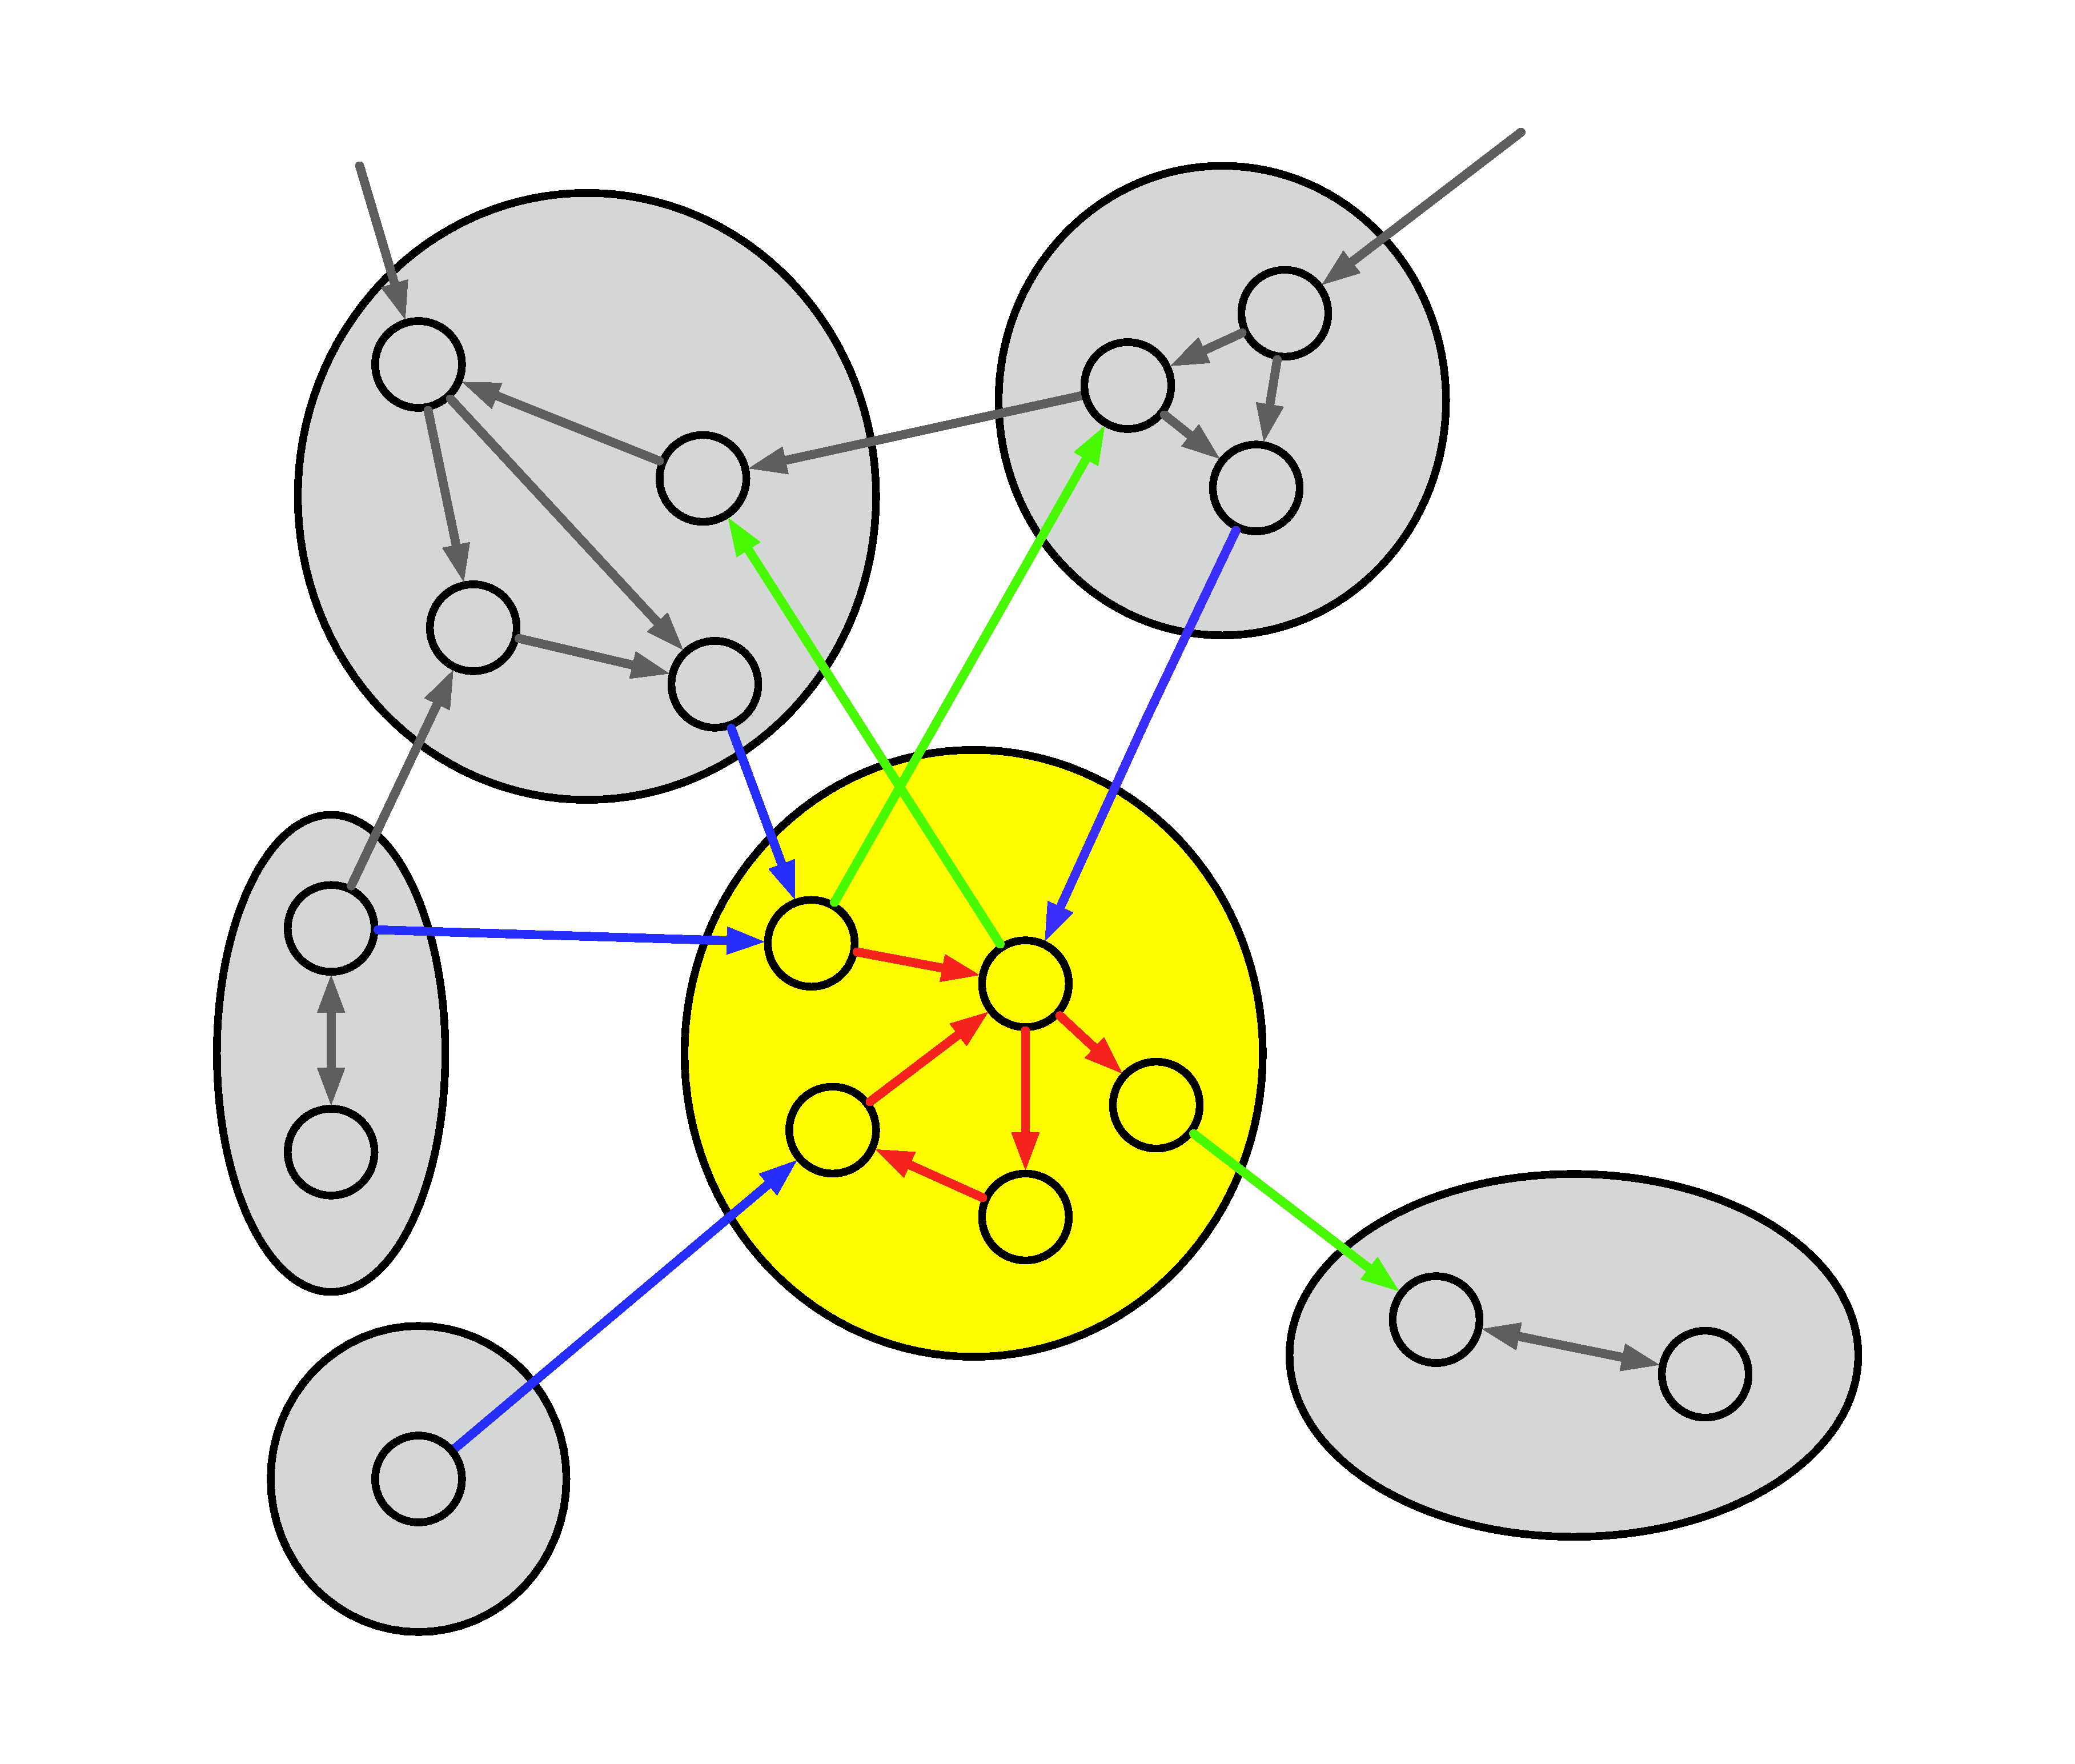
\includegraphics[width=0.50\textwidth]{figures/edge-types.eps}
\caption{An example of the edges considered in determining the edge weight distribution for a given community (the focal community is in yellow). We focus on the internal-to-internal (red), internal-to-external (green), and external-to-internal (blue) edges. For a given focal community, all other edges (grey) are not considered.}
\label{Fig-edge_types}
\end{figure}

For example, Figure~\ref{Fig-edge_types} shows the distributions of hashtag-based weights for the largest community defined by mention-retweets. We see that the distribution of internal-to-internal hashtag weights has a longer tail, with edges 

\begin{figure}[h!]
  \centering
\includegraphics[width=0.50\textwidth]{Figures/comm0_labels-mention-retweet_weights-hashtag-ecdf.pdf}
\caption{The proportion of edges with a weight at least as large as the weight on the horizontal axis, across the types of edges described in Figure~\ref{Fig-edge_types}.}
\label{Fig-dist_across_community}
\end{figure}

\begin{table}
	\caption{The median value for the ratio of the median external/internal-to-internal/external weight to median internal-to-internal weight for the different community/weight pairings.}
	\centering
	\begin{tabular}{c | c | c  c  c  c}
		& & \multicolumn{4}{ c }{Community} \\ \hline
		\multirow{4}{*}{Weight} & & S & TE & MR & HT \\ \hline
		& TE & $0.0 / 0.0$ & $0.0 / 0.0$ & $0.0 / 0.0$ & $0.0 / 0.0$\\
		& MR & $0.0 / 0.0$ & $0.0 / 0.0$ & $0.0 / 0.0$ & $0.0 / 0.0$\\
		& HT & $0.0 / 0.0$ & $0.0 / 0.0$ & $0.0 / 0.0$ & $0.0 / 0.0$
	\end{tabular}
\end{table}
\section{Discussion}

\subsection{Questions Influence Community Structure}
\input{parts/conclusion.tex}

\bibliography{references}
\bibliographystyle{aaai}

\end{document}

\end{document}
